\documentclass[11pt]{article}
 %
\usepackage[utf8]{inputenc}
%                  
%\usepackage[french]{babel} % Pour adopter les règles de typographie française

%\usepackage[T1]{fontenc} % Pour que LaTeX comprenne les caractères accentués ;
                         % norme iso-8859, cela risque de ne pas marcher avec des fichiers créés sous windows
%\usepackage{amsmath,amssymb,amsfonts} % Les bibliothèques LaTeX de l'American Mathematical Society sont pleines de macros intéressantes (voire indispensables).

\pagestyle{headings}  
\usepackage{booktabs} %pour les lignes "excel" dans les tables
\usepackage{float}

\usepackage{array}
\usepackage{graphics,graphicx, makeidx}
%
\usepackage{amsmath}
\usepackage{amsthm}
\usepackage{amsfonts}
\usepackage{amssymb}
\usepackage{ stmaryrd } % pour les délimiteurs d'intervalles un peu complexes
%
%\usepackage{amsmath,amsfonts,mathrsfs}
%\usepackage{theorem}
\usepackage{geometry}
\usepackage{epic,eepic}
\usepackage{times}
\usepackage{pgf}%,pgfarrows,pgfnodes}
\usepackage[absolute,overlay]{textpos}
%\usepackage{hyperref}
\usepackage{xcolor}
\usepackage{verbatim}
\usepackage{graphicx}
%\usepackage{pgfarrows,pgfnodes}
\usepackage{url}
\usepackage{dsfont}
\usepackage{multicol}
\usepackage{xspace}
\usepackage{subfigure}
% pour les en-têtes
\usepackage{fancyhdr}
\pagestyle{fancy}
%
\usepackage{eurosym}
%
\usepackage{algorithm}
%\usepackage{algpseudocode}
\usepackage{algorithmic}
%%%
\geometry{a4paper,textwidth=15cm, textheight=21cm}
%\theoremstyle{plain}
%\newtheorem{exo}{Exercice}
%\newtheorem{quest}{}[exo]
\theoremstyle{plain}% default
\theoremstyle{definition} \newtheorem{lem}{Lemma}[section]
\theoremstyle{definition} \newtheorem{claim}{Claim}[lem]
\theoremstyle{definition} \newtheorem{theorem}{Theorem}[section]


%
\theoremstyle{definition} \newtheorem{exo}{Exercice n$^\circ$}
\theoremstyle{definition} \newtheorem{quest}{}[exo]
\theoremstyle{definition} \newtheorem{sousquest}{}[quest]
%
\theoremstyle{remark}
\newtheorem*{notation}{Notations}
%\newtheorem*{note}{Note}\newtheorem{case}{Case}
%
\theoremstyle{definition}
\newtheorem{defin}{Definition}[section]
%\newtheorem{conj}{Conjecture}[section]\newtheorem{exmp}{Example}[section]
%
\lhead{}
\chead{}
\rhead{}
%
\lfoot{ }
\cfoot{   }
\rfoot{\thepage}
%
\renewcommand{\headrulewidth}{0.4pt}
\renewcommand{\footrulewidth}{0.4pt}
%-------------------------------------
\title{ \bf {A linear formulation for the Synchronous Management of Energy Production and Consumption}}
%       \normalsize \bf Notions de base  $1$}
%\title{ Instance $(T, p, c, A, a(u)=d_T(u), u \in A)$ }
\author{Fatiha Bendali, Eloise Yollande Mole Kamga, Jean Mailfert, Alain Quilliot, Hélène Toussaint\footnote{LIMOS CNRS 6158, Labex IMOBS3, Clermont-Ferrand, France. }}
%\date{July 2019}
%\date{\today}
\date{}
%

\begin{document}
%----------------------------
\maketitle
\thispagestyle{fancy}
%
%--------------------------
{\bf Abstract}
Renewable energies presently appear to be an obvious and efficient solution to fight against climate change. Among these, hydrogen has all the attributes to be the most renewable, clean, efficient and non-toxic form of energy. In this work, we are interested in modeling the synchronization of hydrogen refueling of a vehicle during its pick-up and delivery tour with the production of hydrogen by photolysis and solar heat within a micro-plant. A Mixed Integer Linear Program is provided along with families of strengthening valid inequalities.  A structural study of two families of matching in a bipartite graph are described and as a result,  path constraints are generated. Experimental results show that the linear relaxation is deeply improved by introducing some valid inequalities whereas the mixed integer linear program seems to resist.
  
{\bf Keywords:} Mixed Integer Linear Program, Synchronization, Hydrogen production, Vehicle consumption, Matching, Path polytope. 
%%%%
\section{ Introduction}\label{sec1}
%%%%%%%%%%%%%%%%%%%%%%%%%%%%%%%%%%%%%%%%%%%%%%%%%%%%%%%%%%%%%%%%%%%%%%%%%%%%
Undoubtedly, traditional transport and electricity generation have their share of responsibility in
the climate warming emissions.
OR community is very active on green transportation and deep reflection is conducted about
the optimal uses of renewable energy  \cite{Dekk,Deza,Erdo,Ray}.
Hydrogen does not emit polluting gases during production and is easy to store. However,
its generating cost through electrolysis process is expensive compared to that of fossil fuel
and its high volatility requires extensive safety measures.

In this line of thought are inserted  activities of Labex IMOBS3 program, at Clermont-Ferrand (France),
 devoted to Innovative Mobility. To avoid costly electrolytic techniques, researchers rely on 
solar power and photolysis \cite{Grim,Lich}, which naturally  makes
the productivity of the process deeply dependent on the sun intensity.
This work mixes the control of a micro-plant producing hydrogen with the search of pick-up and delivery tours
for  autonomous
hydrogen-powered vehicles. %the autonomous
%electrical vehicles in charge of pick-up and delivery tours.
Taken as a whole, the problem involves forecasting, safety management and scheduling. Still, since our purpose is to focus on algorithmic features of
\emph{synchronization}, we restrict ourselves to the last issue, and set a simplified Energy Production and Consumption model restricted to the case of 
\emph{one} vehicle required to perform tasks according to a prefixed order  as in \cite{Koc}, periodically going back to the micro-plant in order to refuel. The vehicle starts
its route with some $H_2$ fuel load, and its tank has a limited capacity.
The micro-plant has a limited
production/storage capacity, which depends on solar illumination. Our goal is to synchronize both 
the refueling transactions of the vehicle and the production/storage activity of the
micro-plant while minimizing economical production  cost and the duration of the vehicle tour. This problem is NP-Hard. 
We have proposed in \cite{Bend} a model based on dynamic programming. The 
algorithm  involves a 2D time space which links energy consumption by the vehicle and the production
by the micro-plant. The number of states induced by the dynamic programming procedure becomes an issue as soon
as the size of the problem increases, although  several filtering rules  have been defined. 

In this paper,  a Mixed Integer Linear Programming formulation ($MILP_{SMEPC}$) for the Synchronous Management Energy Production and Consumption problem ($SMEPC$)
is presented. Its linear relaxation  ($RMILP_{SMEPC}$) is shown to have a positive objective value and 
 some valid inequalities are given to strengthen the  linear formulation. 
Moreover,  two families of $\{0,1\}$-variables are highlighted to drive any feasible solution  of $ SMEPC$.
As a consequence, the structural properties of these variables are studied. 
We find that the synchronization of the energy consumption of the vehicle and the energy production by the micro-plant can be associated to 
 matchings in a bipartite graph, characterized by  solutions of a chain polyhedron.
Some numerical experiments are carried out with CPLEX solver that emphasize the efficiency of some of valid inequalities while some others fail to improve the results. 




%%%%%%%%%%%%%%%%%%%%%%%%%%%%%%%%%%%%%%%%%%%%%%%%%%%%%%%%%%%%%%%%%%%%%%%%%%%%
%Some sources of climate warming emissions come from transportation, electricity generation and industry. This gives rise to deep reflexion about the subject of cleaning and using renewable energy.
%A good example is provided by the activities of Labex IMOBS3 program in Clermont-Fd, France,
%devoted to Innovative Mobility. In the context of this project, we are currently involved into
%the control of a micro-plant for hydrogen production, which feeds autonomous vehicles with hydrogen
%fuel. Athough hydrogen does not emit polluting gases during  production and it is easy to store,  its negative aspect is its high cost production through electrolysis instead of fossil fuels and its high volatility which requires extensive safety measures. 
%Thus, while most hydrogen production is usually performed through power costly
%electrolysis processes, researchers rely here on solar power and photolysis \cite{Grim,Lich}, which make
%the productivity of the process deeply depend on the intensity of solar illumination. 
%%According to this paradigm, the energy production/consumption process becomes endogenous, and performed according to a closed loop which requires high synchronization.
%Because of the IMOBS3 project, we deal here with the synchronous management of, on one
%side, a fleet of small electric vehicles provided with hydrogen power cells, and, on the other side, a micro-plant in charge of local hydrogen fuel production. Taken as a whole, the problem involves forecasting, safety management and scheduling. Still, since our purpose is to focus on algorithmic features of synchronization, we restrict ourselves to the last issue, and set a simplified Energy Production and Consumption model restricted to the case of one vehicle required to perform tasks according to a prefixed order while  as in \cite{Koc}, periodically going back to the micro-plant in order to refuel. This vehicle starts
%its route with some $H_2$ fuel load, and its tank has a limited capacity.
%The micro-plant has a limited
%production/storage capacity, which depends on solar illumination. Our goal is to synchronize both the
%the refueling transactions of the vehicle and the production/storage activity of the
%micro-plant while minimizing production economical cost and the duration of the vehicle tour. This problem is NP-Hard. 
%We have proposed in \cite{Bend} a model based on dynamic programming.This 
%algorithm involves a 2D time space which links energy consumption by the vehicle and its production
%by the micro-plant. Since the number of states induced by this algorithm becomes an issue as soon
%as the size of the problem increases, we define several filtering rules for this algorithm. 
%
%In this paper, we present a mixed integer linear programming formulation ($MILP_{SMEPC}$) for the synchronous management energy production and consumption ($SMEPC$). We prove that its linear relaxation  ($RMILP_{SMEPC}$) has a positive objective value and we propose some valid inequalities to strengthen the two linear formulations. In particular, we show that fixing two families of $\{0,1\}$-variables extends to a feasible solution of $ SMEPC$. A consequence of this result led us to study the structural properties of these variables. We find that the synchronization of the energy consumption of the vehicle and the energy production by the micro plant can be associated to a matching in a bipartite graph whose existence is linked to solutions of the chain polytope. Some numerical experiments are carried out with CPLEX solver that show the efficiency of some of valid inequalities while some others fail to improve the results. 
%

%%%%%%%%%%%%%%%%%%%%%%%%%%%%%%%%%%%%%%%%%%%%%%%%%%%%%%%%%%%%%%%%%%%%%%%%%

The remainder of this paper is organized as follows. Section~\ref{sec2} formally introduces the \emph{SMEPC} model. Section~\ref{sec3} describes a MILP formulation of the problem. Section~\ref{sec4} presents theoretical  properties of the linear relaxation as well as some new valid inequalities. Structural properties and
separation procedures are given in Section~\ref{sec5} and computational results are proposed in Section~\ref{sec6}. Finally, Section~\ref{sec7} concludes and outlines research perspectives.
%%%%%%%%%%%%%%%%%%%%%%%%%%%%%%%%%%%%%%%%%%%%%%
\section{Problem description, definitions and notations}\label{sec2}

\subsection{ {\it The model}}

We define the \emph{SMEPC} as follows. A vehicle powered by $H^2$ hydrogen fuel, has to visit a set of stations that need to be served, following a route which begins and ends at a special station: the \emph{Depot}. Close to it, there is a Micro-Plant ($MP$) which is a charging station. The vehicle performs a tour starting from the \emph{Depot} 
(labelled $0$), passing through the sequence of stations $j=1, \ldots, M$ and returning to the \emph{Depot}
 (labelled $M+1$). It leaves the depot at the date $0$ and must return before the date $T_{\textrm{Max}}$.  Travelling from one station $j$ to the next one $j+1$ incurs a driving time $t_j$ that corresponds to the shortest path in time from $j$ to $j+1$ and an energy consumption $e_j$ associated to this path. As the capacity of its tank is limited to $C^{\textrm{Veh}}$, the vehicle may need to periodically refuel between two stations. 
The initial and final quantity of hydrogen in the vehicle's tank is denoted by $E_0$. Going from station $j$ to the Micro-Plant takes a time (resp. an energy consumption) $d_j$ (resp. $\epsilon_j$), whereas the time 
(resp. the  energy consumption) to return from $MP$ to $j$ is denoted by $d^*_{j}$ (resp. $\epsilon^*_{j}$),
see Figure \ref{Notation_inputs}. We consider that the time values and energy ones are non null and satisfy the triangle inequality.\\
%%%%%%
\begin{figure}[!ht]
	\centerline{
		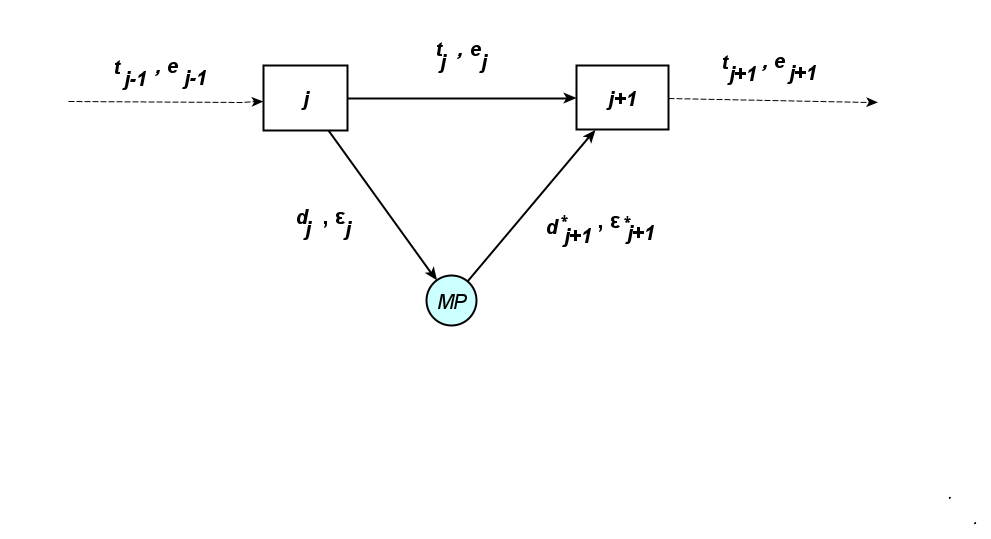
\includegraphics[height=50mm]{Notation.png}}
	\caption[]{Time and Energy symbols between  stations $j$,  $j+1$ and the micro-plant}
	\label{Notation_inputs}
\end{figure}

The micro-plant produces $H^2$ from water through a combination of photolysis and
electrolysis. Resulting $H^2$ is stored inside a tank located directly beside the micro-plant, whose capacity (in
energy units) is denoted by $C^{\textrm{MP}}$. We suppose that:
\begin{itemize}
\item The time space $\{0, 1, 2, \ldots, T_{\textrm{Max}} \}$ is divided into periods $P_i = [p.i, p.(i + 1)[$, for $ i \in \{0, \ldots, N - 1\}$, all with a same length equal to $p$ such that $T_{\textrm{Max}}= N.p$. For the sake of simplicity, we identify index $i$ and period $P_i$. 
\item If the micro-plant is active at some time during period $i$, then it is active during the whole period $i$, and produces $R_i$ hydrogen fuel units, where production rate $R_i$ depends on period $i$. 
\item At time $0$, the current load of the micro-plant tank is equal to $H_0 \le C^{\textrm{MP}}$ and the micro-plant is not active. We impose that the same situation holds at time $T_{\textrm{Max}}$.
\item Because of safety concerns, the vehicle cannot refuel while the micro-plant is producing. Any vehicle refueling transaction should start at the beginning of some period $i \in \{ 0, 1\ldots, N - 1 \}$, and finish at the end of
period $i$ (which means that each refueling operation lasts $p$ units of time). Since vehicle refueling and energy production are mutually exclusive, the vehicle may wait at
the micro-plant before being allowed to refuel.
\end{itemize}

Producing $H^2$ fuel has a cost, which may be decomposed into {\it a fixed activation cost} denoted by $Cost^F$, charged every time the micro-plant is activated and {\it a time-dependent production cost} $Cost^V_i$ which corresponds to the power consumed during period $i$ provided that the micro-plant is active during this period. 

A solution of the SMEPC consists in a plant activity schedule that indicates the periods when the
$H^2$ production happens, a vehicle timetable which specifies the arrival dates at each station
and a refueling policy which provides the energy quantities needed by the vehicle and the stations
from which it will recharge.
%%%%%
%%%%%%%%
%\begin{figure}[!ht]
%	\centerline{
%		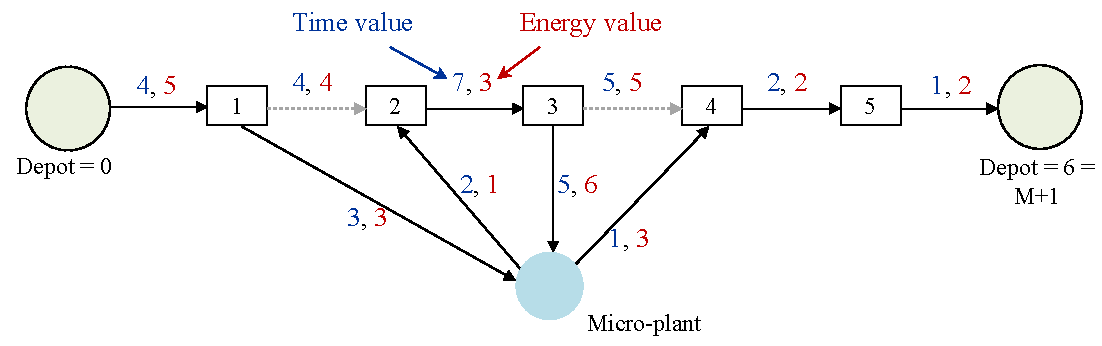
\includegraphics[height=5cm]{EN_Trip.pdf}}
%	\caption[Une tournée de véhicule]{Une tournée de véhicule avec ses opérations de recharge en hydrogène avec $M=5$. }
%	\label{Trip}
%\end{figure}
%%%%%%
%%%%%%%%%
%\begin{figure}[!ht]
%	\centerline{
%		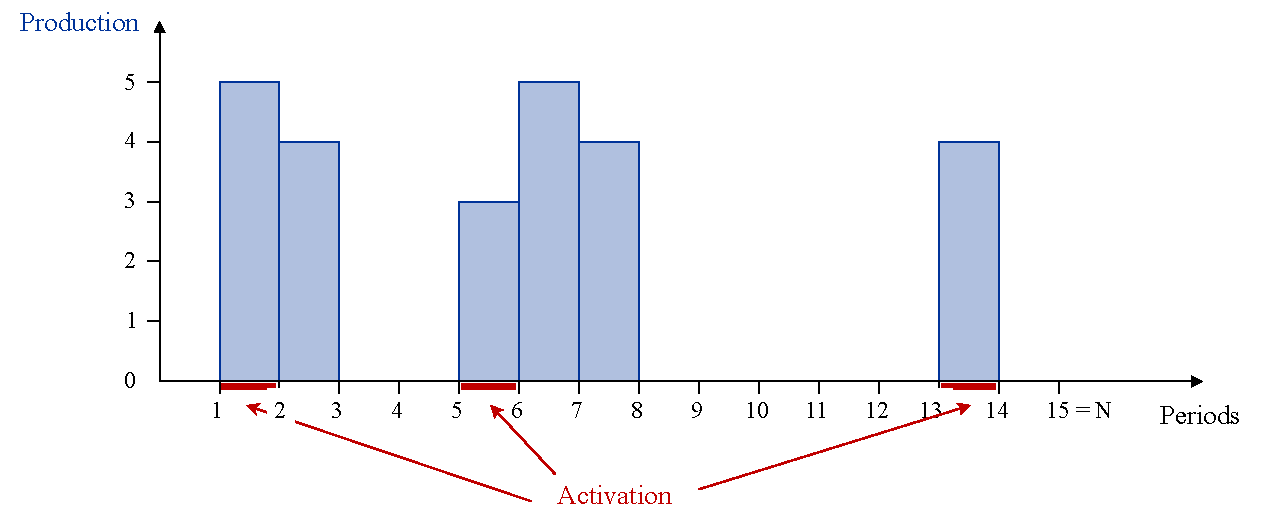
\includegraphics[height=6cm]{EN_exempl_cout_prod.pdf}}
%	\caption[Une stratégie de production]{Un exemple de stratégie de production. }
%	\label{exempl_cout_prod}
%\end{figure}
%%%%%%%%%
%%%%%%%
%\begin{figure}[!ht]
%	\centerline{
%		\includegraphics[height=10cm]{EN_Rendement_cout_prod.pdf}}
%	\caption[Coûts de production]{Coûts de production et rendement en fonction du temps pour la micro-usine de la figure (\ref{exempl_strategie_prod}). }
%	\label{exempl_rendement_prod}
%\end{figure}
%%%%%%%%%%%
\subsection{{\it The objectif}}
The Synchronized Management of Energy Production and Consumption problem ($SMEPC$) consists
in scheduling both the vehicle and the micro-plant in such a way that:
\begin{itemize}
\item The vehicle starts from $Depot = 0$, visits all stations $j = 1,\ldots, M$ and comes back to $Depot=M+1$ at some time $T_{M+1} \in [0, T_{\textrm{Max}}]$, refueling as many times as necessary at the micro-plant ; 
\item The micro-plant produces and stores in time the $H^2$ fuel needed by the vehicle;
\item  Both induced $H^2$ production cost $Cost$ and time $T_{M+1}$ are the smallest possible. The two previous criteria are merged together into a unique one of the form: $Cost + \alpha.T_{M+1}$, where $\alpha$ is a conversion factor from time into  economical cost.
\end{itemize}

%MAIS FINALEMENT C'EST TRES BIEN ECRIT DANS LE RAIRO? ON RECUPERE ?
%%%%%%%%%%%%%%%%%%%%%%%%%%%%%%%%%%%%%%%%%%%%%%%
\section{A Mixed Integer Linear Programming formulation }\label{sec3}
We propose here a mathematical formulation by a linear program with mixed integer variables called $MILP_{SMEPC}$. For the sake of clarity, it will be defined on the basis of the following three elements:
\begin{itemize}
\item Hydrogen production: The Micro-Plant problem,
\item Hydrogen consumption: The vehicle tour problem,
\item Synchronization of consumption and production: The synchronization problem.
\end{itemize}

\subsection {Input for $MILP_{SMEPC}$}
%
\begin{enumerate} 
\item {\bf Vehicle related input}
\begin{itemize}
\item $M$: number of stations ($Depot$ excluded)
\item $\Gamma= (Depot=0, 1, \ldots,M,Depot = M + 1)$: vehicle tour (without refueling)
\item $T_{\textrm{Max}}$: maximal time for the vehicle to achieve its tour
\item $C^{\textrm{Veh}}$: vehicle tank capacity
\item $E_0$: initial vehicle hydrogen load
\item $t_j$: required time to go from station $j$ to station $j + 1$
\item $d_j$: required time to go from station $j$ to the micro-plant
\item $d^*_j$: required time to go from the micro-plant to station $j$
\item $e_j$: required energy to go from station $j$ to station $j + 1$
\item $\epsilon_j$: required energy to go from station $j$ to the micro-plant
\item $\epsilon^*_j$: required energy to go from the micro-plant to station $j$
\end{itemize}
\item {\bf Micro-plant production related input}
\begin{itemize}
\item $N$: number of production periods
\item $p$: duration (in time units) of one production period, $N.p=T_{\textrm{Max}}$
\item $C^{\textrm{MP}}$: micro-plant tank capacity
\item $H_0$: initial micro-plant hydrogen load
\item $Cost^F$: activation cost
\item $P_i = [p.i, p.(i + 1)[$: time interval related to production period $i$
\item $R_i$: production rate related to period $i$
\item $Cost^V_i$: production cost related to period $i$
\end{itemize}
\end{enumerate}
The data above are supposed to be integer.
%
\subsection{Variables and constraints}
We first propose a Mathematical Programming oriented formulation, which allows to clearly identify main variables and constraints.

\subsubsection{Variables}

\begin{enumerate} 
\item [\bf Vehicle:]
When the vehicle travels from a station  $j \in \{  0,\ldots, M \} $ to the next one, we define
\begin{itemize}
\item  a decision variable $x_j \in \{0,1\}$,  such that $x_j = 1$ when the vehicle refuels between $j$ and $j+1$;
\item the refueling time $T^*_j, T^*_j \in \{ 0, p, 2p, \ldots, (N-1)p \}, $  when the vehicle starts to refuel, if $x_j = 1$;
\item the $H^2$ quantity  $L_j, L_j \geq 0 \textrm{ and integer }, $ loaded by the vehicle, if $x_j = 1$.
\end{itemize}
We also consider, when the vehicle arrives at  any station $j \in \{  0,\ldots, M +1 \} $,
\begin{itemize}
\item its arrival time $T_j, T_j  \in \{ 0, 1, 2, \ldots, T_{\textrm{Max}} \}$;
\item the $H^2$ load $V^{\textrm{Veh}}_j, V^{\textrm{Veh}}_j  \geq 0 \textrm{ and integer }$, of its tank.
\end{itemize}

%\begin{itemize}
%\item $x = (x_j, j = 0,\ldots, M)$, with $\{0, 1\}$ values such that $x_j = 1$ when the vehicle refuels while travelling from station $j$ to station $j + 1$;
%
%\item $L = (L_j, j = 0, \ldots, M)$, with non negative integer values such that if $x_j = 1$, then $L_j$ is the $H^2$ quantity loaded by the vehicle while travelling from $j$ to station $j + 1$;
%\item $T = (T_j, j = 0, \ldots, M+ 1)$, with non negative integer values: $T_j$ is the time when the vehicle arrives at station $j$, we have that $T_j \in \{ 0, 1, 2, \ldots T_{\textrm{Max}} \}$;
%\item $T^* = (T^*_j, j = 0, \ldots, M+ 1)$, with non negative integer values such that if $x_j = 1$, $T^*_j$ is the time when the vehicle starts refueling while travelling from $j$ to station $j + 1$, 
%we have that $T^*_j \in \{ 0, p, 2p, \ldots (N-1)p \}$;
%\item $V^{\textrm{Veh}} = (V^{\textrm{Veh}}_j, j = 0, \ldots, M + 1)$, with non negative integer values: $V^{\textrm{Veh}}_j$ is the $H^2$ load of the vehicle tank when the vehicle arrives at $j$.
%\end{itemize}
\item [\bf Production:]
For a period $i \in \{0, \ldots, N-1 \}$, 
\begin{itemize}
\item $y_i \in \{ 0, 1 \}$ depicts whether the micro-plant is activated at the beginning of the period;
\item $ z_i \in \{ 0, 1 \}$ takes the value one if the micro-plant is active along the period;
\item $ \delta_i \in \{0, 1\} $ indicates if the vehicle is refueling during the period;
\item $ L^*_i, L^*_i \geq 0 \textrm{ and integer}, $ is the quantity of $H^2$ loaded by the vehicle during the period in case $\delta_i = 1$.
\item $ V^{\textrm{MP}}_i, V^{\textrm{MP}}_i \geq 0 \textrm{ and integer},$ is the $H^2$ load of the micro-plant tank at the beginning of the period (a fictitious period $N$ is added).

\end{itemize}
\item [\bf Synchronization:]
The meeting point between the vehicle and the plant is the time when the refueling takes place. Thus
we consider
\begin{itemize}
\item the binary variable $U_{i,j}$ which is equal to one  when the vehicle refuels during a period $i, i=0, \ldots, N-1,$ while travelling from a station 
$j, j = 0,\ldots, M, $ to the next one;
\item  the quantity of fuel $m_{i,j}$ given to the vehicle while its travel from station $j$ to $j+1$, at
the period $i$, if $U_{i,j} = 1$.
\end{itemize}
\end{enumerate}

\subsubsection{Constraints}
%
The previous variables are used in a  mixed Integer Linear Program. We explain the way some of those constraints must be understood, specially if they result from  a linearization of logical implications by the Big $M$ technique.

\begin{enumerate} 
\item [\bf Production:]
Let $i$ be a period in $\{  1, \ldots, N - 1 \}$.
\begin{itemize}
\item %At any  period $i $,
The Micro-Plant is \emph{activated} if the production begins whereas 
the micro-plant was shut down at the preceding period.
%$y_i = 1 \rightarrow (z_i = 1 \wedge z_{i - 1} = 0)$ 
The following constraints are obtained. 
\begin{displaymath}
\begin{array}{rlll}
y_i & - z_i & & \leq 0 \\
y_i & & + z_{i - 1}&  \leq 1  \\
-y_i  & + z_i & - z_{i - 1} &\leq 0. %& \textrm{for } i = 1, \ldots N - 1.
\end{array}
\end{displaymath}

\item Production and recharge cannot be carried out simultaneously during a period.
This implies that 
\begin{eqnarray}
 z_i & +\delta_i &  \leq 1. \nonumber
\end{eqnarray}
We also add the initial conditions  $y_0  -z_0  =0 $ and $\delta_0 =0$. %$z_0 = 0$,

\item The storage capacity induces
		$$V^{\textrm{MP}}_{i}\leq C^{\textrm{MP}},$$
		with the initial and final assumptions 
		$V^{\textrm{MP}}_{0}= H_0$ and $V^{\textrm{MP}}_{N} \geq H_0$ (recall that $N$ is a fictitious period).

%\begin{itemize}
%\item $V^{\textrm{MP}}_{0}= H_0$
%\item For any period $i = 1, \ldots, N - 1$: $V^{\textrm{MP}}_{i}\leq C^{\textrm{MP}}$
%\item For any period $i = 1, \ldots, N - 2$: $V^{\textrm{MP}}_{i+1}= V^{\textrm{MP}}_{i}+z_i.R_i -  L^*_i$ such that $L^*_i $, the load of the vehicle during the period $i$, may be nul or at most the capacity of the micro-plant tank: $L^*_i \geq 0$ and $L^*_i \leq  C^{\textrm{MP}}.\delta_i$. 
%\end{itemize}
\item The production of the micro-plant generates flow type equation
	 $$V^{\textrm{MP}}_{i+1}= V^{\textrm{MP}}_{i}+R_i \cdot z_i -  L^*_i.$$
	
\item	The energy $L^*_i $ given by the plant to the vehicle must
be non-negative and smaller than the capacity of the plant tank, that is
$L^*_i \geq 0$ and $L^*_i \leq  C^{\textrm{MP}} \cdot \delta_i$. 

\end{itemize}
\item [\bf Vehicle:]
Assume that $j$ is a station in $\{ 0 \ldots M \}$.
\begin{itemize}
\item Taking into account storage capacity of the vehicle, we have 
$$V_{j}^{\textrm{Veh}}\leq C^{\textrm{Veh}},$$
with the particular conditions at the Depot $V_{0}^{\textrm{Veh}}= E_0 \geq \epsilon_0$ and $V_{M+1}^{\textrm{Veh}}\geq E_{0}$ (the indices $0$ and $M+1$ are assigned to the depot).
%\begin{itemize}
%\item $V_{0}^{\textrm{Veh}}= E_0$
%\item $V_{M+1}^{\textrm{Veh}}\geq E_{0}$
%\begin{itemize}
%\item At any station $j = 1, \ldots, M$:\\
%$V_{j}^{\textrm{Veh}}\leq C^{\textrm{Veh}}$\\
\item The  following set of constraints means that at any time, the vehicle must be able to go to the micro-plant and refuel, and relies on the Triangle Inequality for energy coefficients $e_j$ and $\epsilon_j$
$$V_{j}^{\textrm{Veh}} \geq \epsilon_{j}.$$ 

\item The load of the vehicle verifies a flow type equation
$$V_{j+1}^{\textrm{Veh}}=V_{j}^{\textrm{Veh}}-e_j + (e_j-\epsilon_j-\epsilon^*_{j+1}) \cdot x_j +L_j.$$

\item  The quantity $L_j$ loaded by the vehicle during its travel from $j$ to $j+1$,
if $x_j = 1$,
is subject to: 
\begin{itemize}
\item $L_j \geq 0,$
\item $L_j \leq  C^{\textrm{Veh}} \cdot x_j,$
\item $L_j \leq C^{\textrm{Veh}} + \epsilon_{j}-V_{j}^{\textrm{Veh}}.$ This last inequality
expresses the residual capacity of the vehicle when it arrives at the plant.
\end{itemize}
\item At any station, the time needed to reach the next one 
depends on the choice of 
the trajectory, a direct route or with a deviation through the plant. Thus, we have first
$$T_{j}^*\geq T_j + d_j.$$
%
Moreover, the arrival date $T_{j+1}$ at  station $j+1$ and the time  $T^*_j$ when a refueling is eventually done are linked by  the non linear inequality below.
$$T_{j+1}\geq (1-x_j) \cdot (T_j+t_j)+x_j \cdot (T^*_j+p+d^*_{j+1})$$
Either the vehicle takes the straight road to the next stage or 
the vehicle deviates through the plant. In that case, the next arrival time 
takes into account the waiting time at the tank before refueling.
This can be linearized according to the Big $M$ technique:
 $$T_{j+1}-T_j-t_j\geq -2 T_{\textrm{Max}} \cdot x_j$$
  and 
	$$T_{j+1} -(T^*_j+p+d^*_{j+1}) \geq -2 T_{\textrm{Max}} \cdot (1-x_j ).$$
%\begin{itemize} 
The boundary conditions are
 $T_{0}= 0$ and  $T_{M+1}\leq T_{\textrm{Max}}$.
%\item At any station $ j = 0, \ldots, M$, the time needed to reach the station $j+1$ depends on the choice of trajectory $T_{j+1}\geq (1-x_j) (T_j+t_j)+x_j (T^*_j+p+d^*_{j+1})$.
% which can be linearized by the Big $M$ technique: $T_{j+1}-T_j-t_j\geq -2x_j T_{\textrm{Max}}$  and $T_{j+1} -(T^*_j+p+d^*_{j+1}) \geq -2(1-x_j )T_{\textrm{Max}}$
%\item $T_{j}^*\geq T_j + d_j$
%\end{itemize}
\end{itemize}
\item [\bf Synchronization:]
In order to get a complete formulation, we must explain the way the activities of both the vehicle and the micro-plant are synchronized. We use the synchronization variable $U_{i,j}$ which will tell us, in case the vehicle decides to refuel between a station $j$ and a station $j + 1$, during which period $i$ it will do it.
\begin{itemize}
\item For any station $j$, if the vehicle decides to refuel before going to the following station i.e. $x_j=1$, exactly one period is concerned by this activity: 
$$\sum_{i=0}^{ N-1} U_{i,j}=x_j$$
%
\item If any period $i$ is corresponds to a refueling, that is $\delta_i=1$, then the vehicle comes from a unique  station $j$:
$$\sum_{j=0}^{ M} U_{i,j}=\delta_i$$
\item The  date to reach the micro-plant from a station $j$ is at most the beginning of a period.
This can be expressed by the next non linear inequality 
 $$ \sum_{i=0}^{N-1} p.i.U_{i,j}\geq x_j \cdot (T_j + d_j).$$
This logical constraint can be linearized by: 
$$\sum_{i=0}^{ N-1} p i \cdot U_{i,j}  \geq T_j + d_j - 2 T_{\textrm{Max}}  \cdot (1-x_j)$$
\item The date for refueling between stations $j$ and $j+1$ 
is at least the beginning of a period:
$$\sum_{i=0}^{ N-1} pi \cdot U_{i,j} \le  T^*_j$$
\item The amount of fuel distributed at a period
corresponds to the quantity of fuel loaded during a travel, specifically at a period $i$ that is matched with a station $j$:
 $$L^*_i = \sum_{j=0}^{ M} U_{i,j} \cdot L_j,$$
And symmetrically,
	 $$L_j = \sum_{i=0}^{ N-1} U_{i,j} \cdot L^*_i.$$

To linearize this constraint we
use variables $m_{i,j}$. Hence,
\begin{displaymath}
\begin{array}{lcl}
	L^*_i & = & \sum_{j=0}^{ M} m_{i,j} \\
	L_j & =  & \sum_{i=0}^{ N-1} m_{i,j} \\
	m_{i, j} & \le & C^{\textrm{Veh}} \cdot U_{i,j} \\
	m_{i, j} & \geq & 0.
\end{array}
\end{displaymath}

\end{itemize}
\end{enumerate}
\subsection{The Mixed integer linear formulation $MILP_{SMEPC}$}
\begin{equation}
				\textbf{ Minimize }\sum_{i=0}^{N-1}((Cost^F. y_i) + (Cost_i^V . z_i))+ \alpha .T_{M+1}	\label{Fonction_obj}
	\end{equation}
	%\textbf{ Subject to}\\
	\begin{enumerate}
	\item {\bf Production constraints:}
	\begin{eqnarray}	
	y_0-z_0=0, \delta_0 = 0, &&\label{Prod0}\\
	y_i - z_i \leq 0, & \textrm{ For   } i = 1, \ldots N - 1 ,& \label{Prod1}\\
 y_i + z_{i - 1} \leq 1, & \textrm{ For   } i = 1, \ldots N - 1 , &\label{Prod2}\\
z_i - z_{i - 1}-y_i \leq 0, & \textrm{ For   } i = 1, \ldots N - 1 ,& \label{Prod3}\\
z_i+\delta_i \leq 1, &\textrm{ For }  i= 1, \ldots N-1,&\label{Prod4}\\ 
	V^{\textrm{MP}}_{0}= H_0, & & \label{Prod5} \\
		V^{\textrm{MP}}_{i}\leq C^{\textrm{MP}},  &\textrm{ For  } i = 0, \ldots N-1, &	\label{Prod7}	\\
			V_{N}^{\textrm{MP}}\geq H_{0},&& \label{Prod6}\\
		V^{\textrm{MP}}_{i+1}= V^{\textrm{MP}}_{i}+ R_i \cdot z_i -  L^*_i,  &\textrm{ For }  i = 0, \ldots N-1, &	\label{Prod8}	\\
			 V^{\textrm{MP}}_{i} \geq 0, L^*_i \geq 0, & \textrm{ For }  i = 0, \ldots N-1, &\label{Prod9}\\
			 L^*_i \leq  C^{\textrm{MP}} \cdot \delta_i, & \textrm{ For }  i = 0, \ldots N-1.& \label{Prod10}
		%\end{align}
\end{eqnarray}

%Constraints (\ref{Prod1})-(\ref{Prod3}) express the logical implication: $y_i = 1 \rightarrow (z_i = 1 \wedge z_{i - 1} = 0)$.
\item {\bf Vehicle constraints:}
\begin{eqnarray}	
V_{0}^{\textrm{Veh}}= E_0,  && \label{Prod11} \\
V_{j}^{\textrm{Veh}}\leq C^{\textrm{Veh}},&\textrm {For   } j = 0, \ldots M ,&\label{Prod13}\\
V_{M+1}^{\textrm{Veh}}\geq E_{0},&& \label{Prod12}\\
V_{j}^{\textrm{Veh}} \geq \epsilon_{j},& \textrm{ For }  j = 0, \ldots M,&\label{Prod14}\\
V_{j+1}^{\textrm{Veh}}=V_{j}^{\textrm{Veh}}-e_j + (e_j-\epsilon_j-\epsilon^*_{j+1}) \cdot x_j +L_j,& \textrm{ For  } j = 0, \ldots M ,&\label{Prod15}\\
L_j \geq 0,& \textrm{ For }  j = 0, \ldots M ,&\label{Prod16}\\
 L_j \leq C^{\textrm{Veh}} \cdot  x_j ,& \textrm{ For }  j = 0, \ldots M ,&\label{Prod17}\\
L_j \leq C^{\textrm{Veh}} + \epsilon_{j}-V_{j}^{\textrm{Veh}},& \textrm{ For }  j = 0, \ldots M ,&\label{Prod18}\\
T_{0}= 0,&& \label{Prod19}\\
T_{j}  \geq 0,&\textrm{ For }  j = 0, \ldots M ,& \label{Prod19bis}\\
T_{j+1}-T_j-t_j\geq -2T_{\textrm{Max}} \cdot x_j ,& \textrm{ For }  j = 0, \ldots M ,&\label{Prod20}\\
 T_{j+1} -(T^*_j+p+d^*_{j+1}) \geq -2T_{\textrm{Max}} \cdot (1-x_j ),& \textrm{ For    } j = 0, \ldots M ,&\label{Prod21}\\
T_{j}^*\geq T_j + d_j,& \textrm{ For }  j = 0, \ldots M,&\label{Prod21bis} \\
T_{M+1}\leq T_{\textrm{Max}}.&& \label{Prod22}
		%V^{\textrm{MP}}_{i}&\leq C^{\textrm{MP}},  &\textrm{ For   i = 0, \ldots, N-1} 	\label{Prod7}	\\
		%V^{\textrm{MP}}_{i+1}&= V^{\textrm{MP}}_{i}+z_i.R_i -  L_i,  &\textrm{ For   i = 0, \ldots, N-1} 	\label{Prod8}	\\
			 %L_i &\geq 0, & \textrm{ For   i = 0, \ldots, N-1} \label{Prod9}\\
			 %L_i &\leq  C^{\textrm{MP}}.\delta_i, & \textrm{ For   i = 0, \ldots, N-1}, \label{Prod10}
\end{eqnarray}

%Constraints (\ref{Prod21})-(\ref{Prod21bis}) express the non linear equation:
%$T_{j+1}\geq (1-x_j) (T_j+t_j)+x_j (T^*_j+p+d^*_{j+1})$
\item {\bf Synchronisation constraints:}
\begin{eqnarray}	
%V_{0}^{\textrm{Veh}}&= E_0,  & \label{Prod11} \\
\sum_{i=0}^{ N-1} U_{i,j}=x_j,  & \textrm{ For }  j = 0, \ldots M ,&\label{Prod23} \\
\sum_{j=0}^{ M} U_{i,j} =\delta_i,  & \textrm{ For  } i=0, \ldots N-1,&\label{Prod24} \\
\sum_{i=0}^{ N-1} pi \cdot U_{i,j} \le  T^*_j, &  \textrm{ For }  j= 0, \ldots M,&\label{Prod25} \\
\sum_{i=0}^{ N-1} pi \cdot U_{i,j}  \geq T_j + d_j-2T_{\textrm{Max}} \cdot (1-x_j),&\textrm{ For  } j = 0, \ldots M ,&\label{Prod26} \\
\sum_{j=0}^{  M} m_{i,j} =L^*_i, &  \textrm{ For }  i= 0, \ldots N-1,&\label{Prod27} \\ 
\sum_{i=0}^{  N-1} m_{i,j} =L_j, &  \textrm{ For }  j= 0, \ldots M,&\label{Prod28} \\ 
m_{i,j} \leq C^{\textrm{Veh}}U_{i,j},& \textrm{ For }  i= 0, \ldots, N-1, j = 0, \ldots M, & \label{Prod29} \\ 
%m_{i,j} \leq L_j,& \textrm{ For   i= 0, \ldots, N-1, j = 0, \ldots, M },&\label{Prod29} \\ 
%m_{i,j} \geq L_j -C^{\textrm{Veh}}(1-U_{ij}),& \textrm{ For   i= 0, \ldots, N-1, j = 0, \ldots, M },&\label{Prod30} \\ 
m_{i,j} \geq 0,& \textrm{ For }  i= 0, \ldots, N-1, j = 0, \ldots M .& \label{Prod30}\\
U_{i,j} \geq 0,& \textrm{ For }  i= 0, \ldots, N-1, j = 0, \ldots M .& \label{Prod31}  
\end{eqnarray}

%Constraints (\ref{Prod26}) express the logical implication:
%$x_j=1 \rightarrow \sum_{i=0, \ldots, N-1} p.i.U_{i,j}\geq T_j + d_j, \forall j= 0, \ldots, M$\\
%Constraints (\ref{Prod27})-(\ref{Prod31}) introduce a new variable $m_{i,j}$ and express the non linear equation:
%$ L^*_i = \sum_{j=0, \ldots, M}U_{i,j}L_j, \forall i= 0, \ldots, N-1$
\item {\bf Decision variable constraints:}
\begin{eqnarray}	
%V_{0}^{\textrm{Veh}}&= E_0,  & \label{Prod11} \\
0 \le y_i, 0 \le z_i, 0 \le \delta_i,  & \textrm{ For  } i=0, \ldots N-1,&\label{Dec01} \\
0 \le x_j \le 1,  & \textrm{ For }  j = 0, \ldots M ,&\label{Dec02}
\end{eqnarray}
and 
\begin{eqnarray}	
%V_{0}^{\textrm{Veh}}&= E_0,  & \label{Prod11} \\
y_i \in \{0,1 \} ,  z_i \in \{0,1 \},  \delta_i \in \{0,1 \},  & \textrm{ For  } i=0, \ldots N-1,&\label{Dec03} \\
 x_j \in \{0,1 \} ,  & \textrm{ For }  j = 0, \ldots M .&\label{Dec04} \\
U_{i,j}\in \{0,1 \} ,& \textrm{ For }  i= 0, \ldots, N-1, j = 0, \ldots M .& \label{Dec05}  
\end{eqnarray}

\end{enumerate}
%%%%%%%%%%%%%%%%%%%%%%%%%%
Figure \ref{Trip_exple} gives a feasible solution in case $p = 2, E_0 = 8, H_0 = 4, TMax = 30, Cost^F = 7, C^{MP} = 15, C^{Veh} = 15$, $\alpha= 1$.The global resulting activation cost is $3*7 = 21$. The time T is equal to $30$. The time-dependent production costs in the activation periods are $Cost_1^V=Cost_2^V=1, Cost_5^V=Cost_6^V=Cost_7^V=2, Cost_{13}^V=1$. Thus, the global cost is equal to $21 + 9 + 30 = 60$.
%\begin{figure}[H]
%	\centerline{
%		\includegraphics[height=100mm]{EN_Rendement_cout_prod.pdf}}
%		%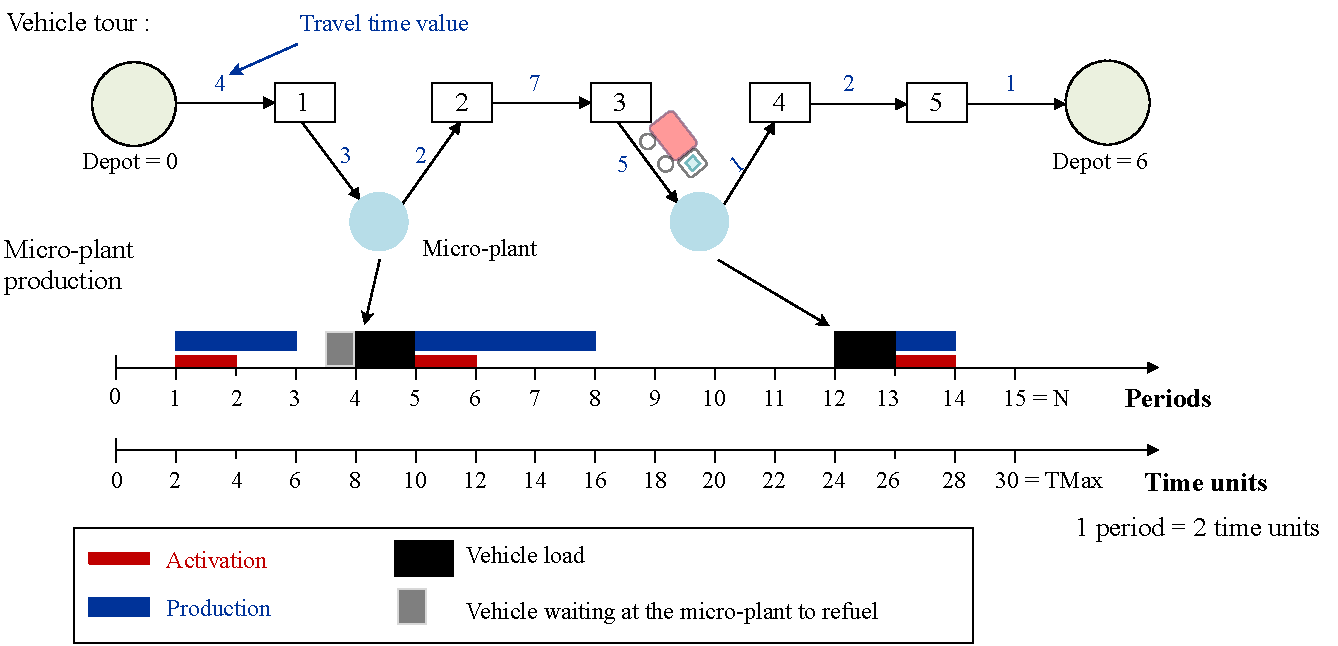
\includegraphics[height=50mm]{EN_synchronisation.pdf}}
%	\caption[]{Activation and time-dependent production costs for the micro-plant }
%	\label{Production}
%\end{figure}
\begin{figure}[H]
	\centerline{
		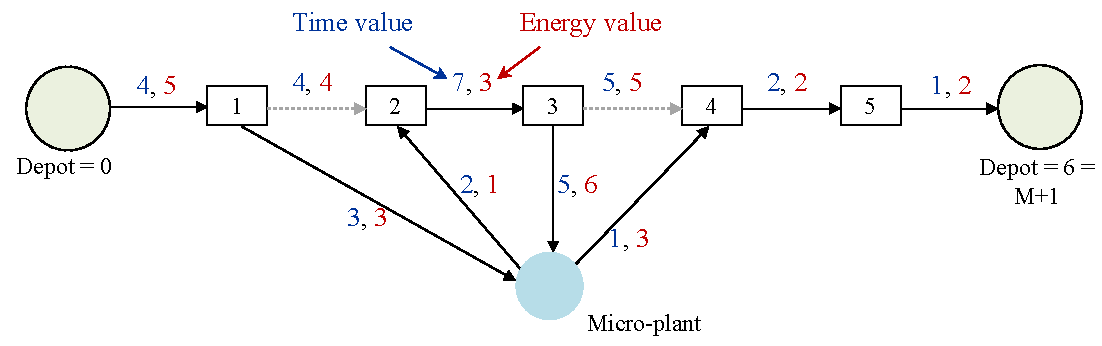
\includegraphics[height=30mm]{EN_Trip.pdf}}
		\centerline{
		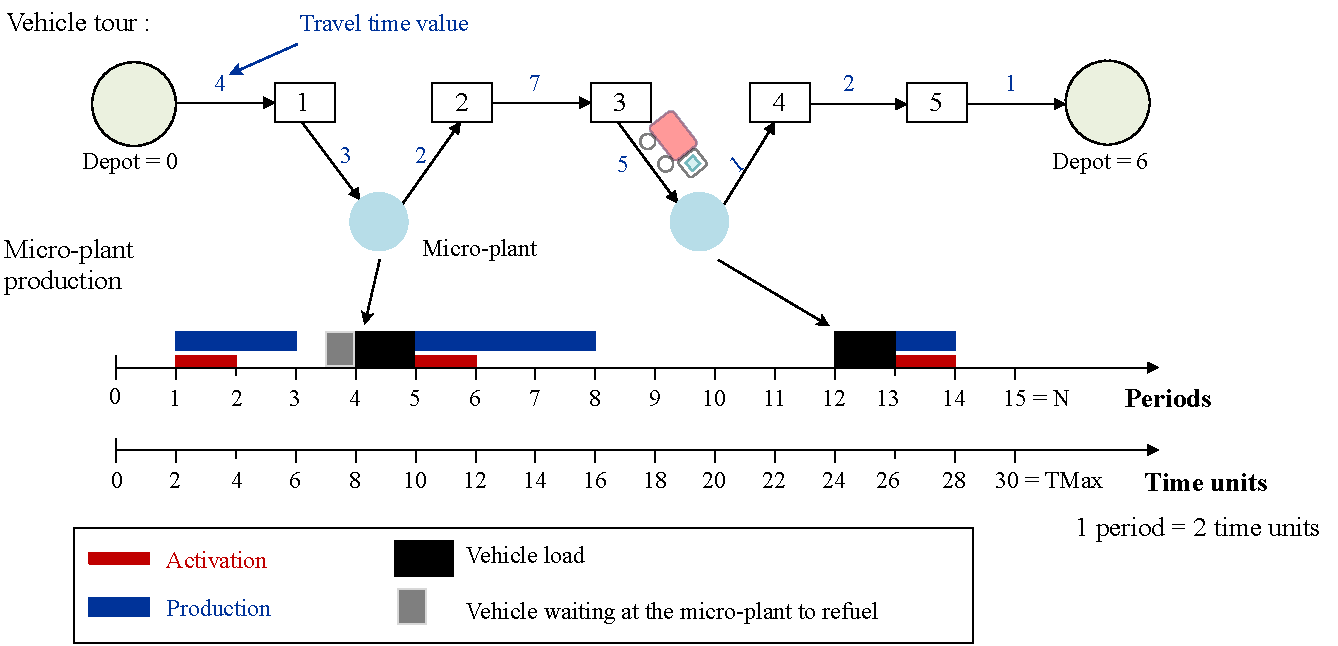
\includegraphics[height=50mm]{EN_synchronisation.pdf}}
	\caption[]{The vehicle pick-up and delivery tour with $M=5$ and its refueling }
	\label{Trip_exple}
\end{figure}
%%%%%%%%%%%%%%%%%%%%%%%%%
\begin{theorem}
$MILP_{SMEPC}$ has a feasible solution if and only if $SMEPC$ has a solution with the same cost.
\end{theorem}
\begin{proof}
Consider an optimal  solution $(\bar{z}, \overline{T}, (\bar{L}, \bar{x}))$ of $SMEPC$,
which describes the plant activity schedule, the vehicle timetable and the refueling policy respectively.
We
check that it can be turned into a feasible solution  of the MILP with the same cost. % comes in a straightforward way. 

%Let $\overline{J} = \{ j_1, \dots j_p \} $ be the set of indices $j \in \{0, \ldots M \}$ for which 
Let $\overline{J}  $ be the set of indices $j \in \{0, \ldots M \}$ for which 
 $x_j $ takes value one. By applying~(\ref{Prod11}) and (\ref{Prod15}), 
the $H^2$ load $\overline{V}^{\textrm{Veh}}$ is iteratively calculated in the following way:
if $ j \in \overline{J}$, then 
$\overline{V}^{\textrm{Veh}}_{j+1} = \overline{V}^{\textrm{Veh}}_{j} - \epsilon_j + \overline{L}_j - \epsilon^*_{j+1}$, else $\overline{V}^{\textrm{Veh}}_{j+1} = \overline{V}^{\textrm{Veh}}_{j} - e_j$.

As the vehicle directly goes to the station after recharging which takes one period of time, 
$ \overline{T}^*$ can be chosen such that
$$ \overline{T}^*_j = \overline{T}_{j+1} - d^*_{j+1} - p \textrm{ and }
 \overline{T}^*_j \in \{0, p, \ldots (N-1)p \}, \textrm{ for } j \in \overline{J}.$$
When $ j$ does not belong to $\overline{J}$, $ T^*_j $ can take any non negative value.
The validity of the vehicle's route means that the vectors $\overline{T} \textrm{ and } \overline{T}^* $ verify
 (\ref{Prod19})-(\ref{Prod22}).

Moreover, an index $\hat{\imath}(j)$ can be assigned to each $j$ in $\overline{J}$,  by taking  $\hat{\imath}(j) \cdot p = \bar{T}^*_j$.
%since $ \overline{T}^*_j \in \{0, p, \ldots (N-1)p \}, \textrm{ for all } j \in \bar{J}$. 
Let $\overline{I} = \{ \hat{\imath}(j): j \in \overline{J} \}$.
One can  assume that
$\delta_i = 1, L^*_i = L_j $ for $i \in \overline{I}$, and $\delta_i =  L^*_i = 0 $ otherwise. 
Similarly, $U_{i,j} = 1 $ if $i =\hat{\imath}(j), j \in \overline{J} $, and $U_{i,j}  = 0 $ otherwise.

Let $\overline{I}^A = \{ i \in \llbracket 0, N-1\rrbracket: \bar{z}_i =1 \} $. $\overline{I}^A$ can be partitioned
into disjoint intervals of the form $[f_k, g_k], k =1, \ldots q  $, on which the plant is active. 
Note than $\bar{z}_{{f_k}-1} = 0 = \bar{z}_{{g_k}+1}$, if  $f_k >0, g_k < N-1, 1 \le k \le N-1 $.
As the micro-plant cannot be active while the vehicle refuels, 
$\overline{I} \cap \overline{I}^A = \emptyset$; this implies that (\ref{Prod4}) is satisfied.

Let us define
\begin{displaymath}
\bar{y}_i = 
\left\{ \begin{array}{cl}
1 & \textrm{if } i = f_k, \textrm{ for some } k \le q, \\
0 & \textrm{otherwise.}
\end{array} \right.
\end{displaymath}
(\ref{Prod0})-(\ref{Prod3}) are  therefore verified by $\bar{y}$ and $\bar{z}$. 
From~(\ref{Prod5}), iteratively applying   equation~(\ref{Prod8})  enables us to determine 
the volume $V^{\textrm{MP}}_{i}, \textrm{ for } i=0, \ldots N-1$. All other inequalities are 
capacity constraints that are necessary satisfied by a feasible solution of  $SMEPC$.


%We only need to follow the trajectory induced by $(\bar{y},\overline{\delta},\bar{x},\bar{L})$ and compute $$(\bar{z},\overline{L^*},\overline{T},\overline{T^*}, \overline{V^{\textrm{Veh}}},\overline{V^{\textrm{MP}}},\overline{U})$$ accordingly.\\
%%%%%%%%%%%%%%%%%%%%%%%%%%%%%%%%%%%%%%%%%%%%%%%%%%%%%%%%%%%%%%%%%%%%%%%%%%%%%%%%%%%%%%%%%%%%%%
%----------------------------------------------------------------------------------------

%From $\bar{y}$ and $\overline{\delta}$ in any period $i$ we can deduce $\bar{z}_i$: if $\bar{y}_i=1$ then from constraints (\ref{Prod1}) and (\ref{Prod2}), $\bar{z}_i=1$ and $\bar{z}_{i-1}=0$( in the same time we have that as $\bar{z}_i=1$ then  necessarily $\bar{y}_{i+1}=0$ from (\ref{Prod2}) ). Constraints (\ref{Prod3}) give $\bar{z}_{i+1}\le 1$. By (\ref{Prod4}) and $\overline{\delta}$, $\bar{z}_{i+1}=0$  if $\overline{\delta}_{i+1}=1$.
%
%From $(\bar{x},\bar{L})$ and  constraints ((\ref{Prod11})-(\ref{Prod18})) we can deduce the load of the vehicle at each station $ \overline{V^{\textrm{Veh}}}$. While $(\bar{x})$ and inequalities ((\ref{Prod19})-(\ref{Prod22})) and ((\ref{Prod25})-(\ref{Prod26})) give the ordered values $\overline{T},\overline{T^*}$ such that $T_{j+1} \ge T_j +t_j$ if $x_j=0$ and $T^*_{j} \ge T_j +d_j$ otherwise. 
%
%From $\bar{x}$ and $\overline{\delta}$ and matching constraints ((\ref{Prod23})-(\ref{Prod24})) we can deduce $\overline{U}$ and $\overline{L^*}$ such that: 
%
%$\overline{U}_{i,j}= 0$ for each $i=0\ldots N-1$ if $\bar{x_j}=0$ while if $\overline{\delta_i}=0$ then $\overline{U}_{i,j}= 0$ for each $j=0\ldots M$ and by (\ref{Prod28})and (\ref{Prod27}), $\overline{L^*_i}=0$
%
%If $\overline{\delta_i}=1$ then by summing constraints (\ref{Prod28}) and using constraints (\ref{Prod24}) we deduce $\overline{L^*_i} \le C^{\textrm{Veh}}$. Moreover, there exists a station $j(i) in \{0,\ldots, M \}$ where the vehicle refuels during the period $i$ so $\bar{x_{j(i)}}=1$ which aims to obtain $\overline{U}_{i,j(i)}= 1$ and $\overline{U}_{i,j}= 0, j \ne j(i)$.
%
%------------------------------------------------------------------------------

%%%%%%%%%%%%%%%%%%%%%%%%%%%%%%%%%%%%%%%%%%%%%%%%%%%%%%%%%%%%%%%%%%%%%%%%%%%%%%%%%%%%%%%%%%%%%

Conversely, let us consider some optimal feasible solution $$(\bar{y},\overline{\delta},\bar{x},\bar{L},\bar{z},\overline{L}^*,\overline{T},\overline{T}^*, \overline{V}^{\textrm{Veh}},\overline{V}^{\textrm{MP}},\overline{U})$$ of the above $MILP_{SMEPC}$.

 By Constraints ((\ref{Prod23})-(\ref{Prod24})), the vector $\overline{U}$ defines a matching $j \rightarrow \hat{\imath}(j)$
between the sets $\bar{J}=\{j \in \{0, \ldots,M\}: \bar{x}_j=1 \} $ and
$\bar{I}=\{i \in \{0, \ldots,N-1\}: \overline{\delta}_i=1 \}$. 
This matching is consistent with the standard linear ordering: 
if $j_1 < j_2$ then $\hat{\imath}({j_1}) < \hat{\imath}({j_2})$. 
Indeed, inequalities (\ref{Prod19})-(\ref{Prod22}) insures that $T_{j+1} > T_j, \forall j$
and $T_{j+1} > T^*_j > T_j, \forall j \in \bar{J}$. Hence 
$T^*_{j_2} > T_{j_2} \geq T_{j_1+1} > T^*_{j_1} $.
From (\ref{Prod25})-(\ref{Prod26}), we derive that $\hat{\imath}({j_2}) p > T_{j_2} >  T^*_{j_1} \geq \hat{\imath}({j_1}) p$.
Therefore, $\hat{\imath}({j_1}) < \hat{\imath}({j_2}) $.

By optimality of the solution, constraints (\ref{Prod20}), (\ref{Prod21}) and (\ref{Prod25}) are tight. 
Thus $\overline{T}$ defines a vehicle timetable. As $L^*_{\hat{\imath}(j)} = L_j, j \in \bar{J}$
 from~(\ref{Prod27})-(\ref{Prod30}),  the vehicle and the micro-plant tanks
have feasible volumes due to flow type and capacity constraints.

We conclude that a solution to the $SMEPC$ 
%$((\bar{x},\bar{L}),\bar{z},\overline{T})$
can be extracted from the optimal feasible solution of the $MILP$, both of
the same cost. 

%This last point derives from inequalities ((\ref{Prod19})-(\ref{Prod22})) and ((\ref{Prod25})-(\ref{Prod26})) which fixe the values $\overline{T}$ and $\overline{T^*}$ such that $T_{j+1} \ge T_j +t_j$ if $x_j=0$ and $T^*_{j} \ge T_j +d_j$ otherwise. If $i_1,i_2$ are consecutive in  $\tilde{I}$ and such that $j(i_1) >j(i_2)$, then we get, by propagating ((\ref{Prod19})-(\ref{Prod22})), $T^*_{j(i_1)} \ge T^*_{j(i_2)}$ which contradicts ((\ref{Prod25})-(\ref{Prod26})).
\end{proof}

%%%%%%%%%%%%%%%%%%%%%%%%%%%%%%%%%%%%%%%%%%%%%%%
\section{Linear relaxation }\label{sec4}

Denote by $RMILP_{SMEPC}$ the linear relaxation of $MILP_{SMEPC}$, i.e. the linear program described by (\ref{Fonction_obj})-(\ref{Dec02})
and by $\bar{Z}_{r}$ its optimal value.
Often, Big~$M$ techniques induce very weak linear relaxations. But here we have the following.

\begin{lem}
If $RMILP_{SMEPC}$ is feasible, then $\bar{Z}_{r} > 0$.
\end{lem}
\begin{proof}
Suppose on the contrary that there is an optimal solution
 $$(\bar{y},\overline{\delta},\bar{x},\bar{L},\bar{z},\overline{L}^*,\overline{T},\overline{T}^*, \overline{V}^{\textrm{Veh}},\overline{V}^{\textrm{MP}},\overline{U})$$
of the $RMILP_{SMEPC}$ such that $\bar{Z}_{r} = 0$.
Necessarily 
\begin{eqnarray*}	
%V_{0}^{\textrm{Veh}}&= E_0,  & \label{Prod11} \\
\bar{y}_i = \bar{z}_i = 0,  & \textrm{ for  } i=0, \ldots N-1.
\end{eqnarray*}
Then from~(\ref{Prod8}) we obtain that $V^{\textrm{MP}}_{i+1}= V^{\textrm{MP}}_{i} -  L^*_i,  \textrm{ for }  i = 0, \ldots N-1	$.
By~(\ref{Prod5}) and (\ref{Prod6}), $  L^*_i =0,  \textrm{ for }  i = 0, \ldots N-1$.
(\ref{Prod27})  implies that  $ m_{i,j} =0 ,   \textrm{ for } j=0, \ldots   M,  i= 0, \ldots N-1$.
 By~(\ref{Prod28}),  $L_j = 0,   \textrm{ for }  j= 0, \ldots M $.
Henceforth, (\ref{Prod15}) gives 
$V_{j+1}^{\textrm{Veh}} < V_{j}^{\textrm{Veh}}, \textrm{ for  } j = 0, \ldots M $.
But this contradicts the initial and final conditions~(\ref{Prod11}) and~(\ref{Prod12}).                   
\end{proof}
%
\subsection{Additional constraints}
Several constraints can be added for strengthening the linear relaxation. 
To achieve this objective we introduce the following data.

For any $j =1, \dots, M$, we set:

$D_j=\sum_{k=0}^{j-1} t_k+d_j$: the earliest arrival time at the micro-plant for a first refueling after  station $j$.

 $D^*_j= d^*_{j+1} +\sum_{k={j+1}}^{M} t_k$: the latest time to finish the trip after refueling at station $j$.

$\tau_m(j) =\lceil \frac{D_j}{p} \rceil$: the earliest period of  a possible refueling at  station $j$;

$\tau_M(j)= N-1 - \lceil \frac{D^*_j}{p} \rceil$: the latest period of a possible refueling at  station $j$;
%Consider the weighted directed digraph $D_1=(V,A)$ built as follows.
%$$V=\{v_{ij}=(i,j) : 0\le j\le M; 0\le i\le N-1\} \cup \{0,M+1\}$$
%$$A=\{(v_{ij},v_{i'j'}) : j<j' \textrm { and } i>i'\}$$
%
\subsubsection{Simple Time constraints}
The inequalities
\begin{eqnarray}
 T_{j+1}^* \geq T_j^*  , & j=0,\ldots M, & \label{temps_veh_rech} \\
 T_{j+1} \geq T_j + t_j + x_j (d_j +d^*_{j+1} - t_j),& j=0,\ldots M, &\label{temps_veh_bis}
\end{eqnarray}
are straightforwardly seen to be valid for $MILP_{SMEPC}$. 
(\ref{temps_veh_rech}) and  (\ref{temps_veh_bis})
insure that the times form  non decreasing sequences. 
We will see in the experimental results that these constraints are very useful.

%
%%%%%%%%%%%%%%%%%%%%%%
%%%%%%%%%%%%%%%%%%%%%%
\subsubsection{Energy constraints}

\begin{eqnarray}
 L_j \geq x_j (\epsilon_j +\epsilon_{j+1}^* - e_j) ,&  j=0, \ldots M. & \label{rech_veh_bis} 
\end{eqnarray}
By considering~(\ref{rech_veh_bis}), the vehicle leaving any station
will arrive at the next one with more hydrogen after a refueling than if it  followed the direct route between the two.

\begin{eqnarray}
 U_{i, j }  = 0  &  i< \tau_m(j) \textrm{ or } i > \tau_M(j) & j=0, \ldots M.  \label{struct_const} 
\end{eqnarray}
Inequalities~(\ref{struct_const}) simply reflect the definitions of $\tau_m(j)$ and $\tau_M(j)$, for any $j$.


\begin{eqnarray}
 \sum_{i=0}^{\tau_M(j)} L_i^*   \geq  & \sum_{k=0}^{j} L_k  ,&  j=0, \ldots M.  \label{rech_veh_mp} 
\end{eqnarray}
(\ref{rech_veh_mp}) expresses the fact that the total quantity refuelled by the vehicle at station~$j$ does not exceed the
total quantity of hydrogen given by the micro-plant till $\tau_M(j)$.

(\ref{rech_veh_mp}) has the following consequences.

Let $F_{j+1}= F_j+e_j+x_j(\epsilon_j+\epsilon^*_{j+1}-e_j)$ with $F_0=0$. $F_{j}$ is the energy used by the vehicle from $0$ to $j$.
 
From~(\ref{Prod8}) and (\ref{Prod15})
\begin{eqnarray}
V_{j+1}^{\textrm{Veh}} & = &  E_0 - F_{j+1} + \sum_{k=0}^{j} L_k, \nonumber \\
V^{\textrm{MP}}_{\tau_M(j)+1} & = &  H_0 + \sum_{i=0}^{\tau_M(j) }  R_i \cdot z_i -  \sum_{i=0}^{\tau_M(j)} L^*_i,  \nonumber	
\end{eqnarray}
for any $j = 0, \ldots M$.

Hence
\begin{eqnarray}
 E_0  + \sum_{k=0}^{j} L_k & \geq &   F_{j+1}, \nonumber \\
H_0 + \sum_{i=0}^{\tau_M(j) }  R_i \cdot z_i & \geq  &  \sum_{i=0}^{\tau_M(j)} L^*_i,  	\nonumber	
\end{eqnarray}
 for  any $ j = 0, \ldots M $. 

Thus we obtain:

\textbf {EC1}: 
\begin{eqnarray}
%F_{j}-E_0 \le \sum_{k<j} L_k& j=0,\ldots M, & \label{EC1-1} \\
\sum_{i=1}^{\tau_M(j)} R_i z_i  & \ge  F_{j+1}-E_0-H_0 & j=0,\ldots M,  \label{EC1-1} \\
\sum_{i=1} ^{N-1} R_i z_i  & \ge   F_{M+1}. &\label{EC1-2} 
\end{eqnarray}

The binary variable $y_i$ is equal to $1$ when the micro-plant is activated at period $i$.
Thus the value $\sum_{i=0}^{\tau_M(j)} y_i$ indicates the number of production intervals between 
the periods $0$ and $\tau_M(j)$. During each of these intervals, the $H^2$ production
cannot exceed the capacity of the micro-plant. Hence
$$ \begin{array}{lclr}
C^{\textrm{MP}} \sum_{i=0}^{\tau_M(j)} y_i & \geq & \sum_{i=0}^{\tau_M(j)} R_i z_i  & j=0,\ldots M.
\end{array}
$$
From~(\ref{EC1-1}), this implies that

\textbf {EC2}:
\begin{eqnarray}
C^{\textrm{MP}} \cdot \sum_{i=0}^{ \tau_M(j)} y_i \ge & F_j - E_0 - H_0 & j=0,\ldots M,  \label{EC2-1} \\
C^{\textrm{MP}} \cdot \sum_{i=0}^{ N-1} y_i  \ge & F_{M+1}.  \label{EC2-2} 
\end{eqnarray}


In a same way, from~(\ref{Prod10}), 
\begin{eqnarray}
\sum_{i=0}^{\tau_M(j)} C^{\textrm{MP}} \cdot \delta_i  \geq  \sum_{i=0}^{\tau_M(j)} L^*_i, & \textrm{ For }  j = 0, \ldots M.& \nonumber
\end{eqnarray}

Therefore we get

\textbf {EC2'}:
\begin{eqnarray}
C^{\textrm{MP}} \cdot \sum_{i=0}^{ \tau_M(j)} \delta_i \ge & F_j - E_0 & j=0,\ldots M,  \label{EC2-11} \\
C^{\textrm{MP}} \cdot \sum_{i=0}^{ N-1} \delta_i  \ge & F_{M+1}.  \label{EC2-22} 
\end{eqnarray}


Similarly to (\ref{rech_veh_mp}), it can be  seen that 
\begin{eqnarray}
 \sum_{i=\tau_m(j)}^{N-1}  L_i^*   \geq  & \sum_{k=j}^{M} L_k  ,&  j=0, \ldots M.  \label{rech_veh_MP} 
\end{eqnarray}
(\ref{rech_veh_MP})  expresses the fact that the total quantity refuelled by the vehicle from station~$j$ does not exceed the
total quantity of hydrogen given by the micro-plant from $\tau_m(j)$. It could be also used for
generating inequalities similar to those of  type~(\ref{EC1-1}) and~(\ref{EC2-1}).


Finally some cover inequalities are proposed.
First, let $ \mu^0_{j}= \sum_{k=0}^{j-1} e_k+ \epsilon_{j}$, for any $j=1, \dots M$.
$ \mu^0_{j} $ represents the   energy consumption of the vehicle starting at the $Depot$ and finishing at the micro-plant before refueling at station $j$.
Next,  $\mu^*_{j}= \epsilon ^*_{j+1} +\sum_{k=j+1}^{M} e_k$, $j=0, \dots, M$. 
$\mu^*_{j}$ is the energy consumption of the vehicle starting at the micro-plant after a refueling at $j$ and finishing at the $Depot$.
%Lastly, for any pair $j_1$, $j_2$ such that $j_1 <j_2$, 
%let $\mu_{j_1, j_2}= \epsilon^*_{j_1+1} + \sum_{j=j_1+1}^{j_2-1} e_j+ \epsilon_{j_2}$ be the energy consumption of the vehicle between two stations $j_1$ and $j_2$ starting and finishing at the micro-plant.
Depending of the fact that the minimal consumption of the vehicle exceeds the initial amount of
hydrogen or the capacity of its tank, the following constraints can be obtained.

\textbf {EC3}:
\begin{eqnarray}
\sum_{k=0}^{ j} x_k   \ge & 1, & j=0,\ldots M, \textrm{ such that } \mu^0_{j} > E_0, \label{EC3-1} \\
\sum_{k=j+1}^{ M} x_k \ge & 1, & j=0,\ldots M, \textrm{ such that } \mu^*_{j} > C^{\textrm{Veh}} - E_0.  \label{EC3-2} 
\end{eqnarray}


%From~(\ref{Prod8}) and (\ref{Prod15})
%\begin{eqnarray}
%V_{j+1}^{\textrm{Veh}} & = &  E_0 - F_{j+1} + \sum_{k=0}^{j} L_k, \nonumber \\
%V^{\textrm{MP}}_{\tau_M(j)+1} & = &  H_0 + \sum_{i=0}^{\tau_M(j) }  R_i \cdot z_i -  \sum_{i=0}^{\tau_M(j)} L^*_i,  \nonumber	
%\end{eqnarray}
%for any $j = 0, \ldots M$.
%Hence
%\begin{eqnarray}
 %E_0  + \sum_{k=0}^{j} L_k & \geq &   F_{j+1}, \nonumber \\
%H_0 + \sum_{i=0}^{\tau_M(j) }  R_i \cdot z_i & \geq  &  \sum_{i=0}^{\tau_M(j)} L^*_i,  	\nonumber	
%\end{eqnarray}
 %for  any $ j = 0, \ldots M $. 
%As a consequence we obtain:

%
%%%%%%%%%%%%%%%%%%%%%%
%%%%%%%%%%%%%%%%%%%%%%
\section{Structural study}~\label{sec5}
%
\subsection{Principal variables}
%
Among all unknowns, the decision variables $(z_i)_{0 \leq i \leq N-1}$ and $(U_{i, j})_{0 \leq j \leq M, 0 \leq i \leq N-1 }$
play a central role.

Indeed, assume that feasible $(z_i)$ and $(U_{i, j})$ are given. Then, by applying~(\ref{Prod23}) and~(\ref{Prod24}),
$(x_j)$ and $(\delta_i)$ are determined, and in consequence, the compatibility of  $(z_i)$ and $(U_{i, j})$
is checked with~(\ref{Prod4}). Next, the $(y_i)$ which indicate the activation of the micro-plant are simply calculated
from~(\ref{Prod0})-(\ref{Prod3}). 

Thus, we obtain two flow-models, (\ref{Prod5})-(\ref{Prod10}) for managing the plant and
(\ref{Prod11})-(\ref{Prod18}) for the evolution of the vehicle tank. These two systems
are synchronized through the variables $(m_{i, j})$ within (\ref{Prod27})-(\ref{Prod30}) and
the schedule is sequentially calculated by (\ref{Prod19})-(\ref{Prod22}), (\ref{Prod25})-(\ref{Prod26}).

These remarks endorse the fact that $(z_i)$ and $(U_{i, j})$ are the principal variables
of our formulation. So we believe that any inequality involving these variables 
could improve the linear relaxation.


%\subsection{Matchings}

In the following, the complete bipartite graph $G=(I+J, E)$ is used where the vertices can be partitionned into two independent sets $I$ and $J$ with $I=\{0,1, \dots,N-1\}$ and $J=\{0,1, \dots,M\}$ and  the set of edges $E=\{ (i, j ): 0 \le i \le N-1, 0 \le j \le M \}$.
%
\subsection{ Non-crossing matchings}\label{Non_crossing_matchings}
We say that two edges $(i,j)$ and $(i',j')$ of a matching in $G$ are crossing if $j<j'$ and $i >i'$. A matching $C$ is called {\it non-crossing} if $C$ has no crossing pair of edges.

 Let $(z_i)$ and $(U_{i, j})$ be a feasible solution of $MILP_{SMEPC}$.
By ~(\ref{Prod23}) and~(\ref{Prod24}), the edge set $C(U)=\{ (i,j) : U_{i, j}=1, 0 \leq j \leq M, 0 \leq i \leq N-1 \}$ is a matching in $G$. Moreover,
 due to the time constraints (\ref{Prod19})-(\ref{Prod22}) and (\ref{Prod25})-(\ref{Prod26}), the matching $C(U)$ has no crossing pair of edges. 

Thus, we aim to search valid constraints for non-crossing matchings.


We associate to $G$ an acyclic digraph $H=(V(H), A(H))$ as follows.
\begin{itemize}
\item[] $V(H)= \{ \{i, j ): 0 \le i \le N-1, 0 \le j \le M \}$,
\item[] The edge set $A(H)$ contains the arcs of the form $((i, j), (i,j-1)), \textrm{ for } 1 \le j \le M, 0 \le i \le N-1$ and
$((i, j), (i+1,j)), \textrm{ for }  0 \le i \le N-2,  0 \le j \le M$.
%
\end{itemize}
Note that $V(H) = E(G)$, and the vertices $(0,M)$ and $(N-1, 0)$ are the sink and the tank of $H$, respectively.
All maximal paths in $H$ are of length $N+M-1$. Denote by ${\cal P}$ the set of all maximal paths in $H$
and by $E(P)$ the edges of $E$ that correspond to vertices of $P$, for $P \in {\cal P}$ .

The graph $H$ induces an order $\preceq$ on the vertices of $V(H)$ so that $(i_1,j_1)\preceq (i_2,j_2)$ if $(i_2,j_2)$ is reachable in $H$ from $(i_1,j_1)$

Given a maximal path $P \in {\cal P}$,  the constraint 
\begin{eqnarray}
 \sum_{(i, j) \in E(P)} U_{i,j} \le 1 &\label{clique_antag_P}
\end{eqnarray}
is called the {\it antagonistic} constraint associated to $P$. 
%%%%%%
\begin{figure}[!ht]
	\centerline{
		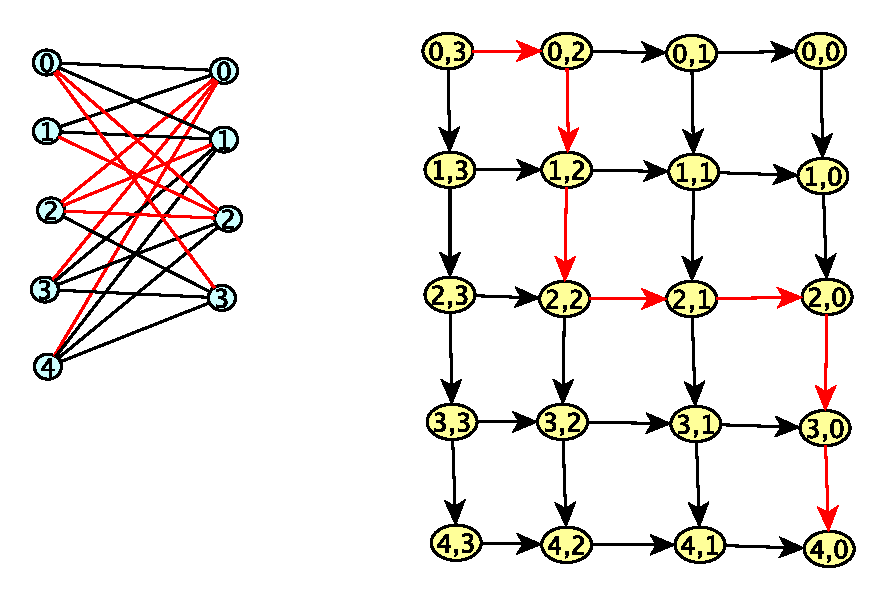
\includegraphics[height=50mm]{NonCrossingM.pdf}}
	\caption[]{A path in $H$ associated to a set of crossing edges in $G$.}
	\label{NCM}
\end{figure}
\begin{lem}\label{lem_antcste}
For any maximal path $P$ in $H$, the antagonistic constraint induced by $P$ is valid for $MILP_{SMEPC}$.
\end{lem}
\begin{proof}
Consider a maximal path $P =( (i_1, j_1), (i_2, j_2), \dots (i_{N+M-1}, j_{N+M-1}), (i_{N+M}, j_{N+M}))$ of ${\cal P}$
with $(i_1, j_1)=(0,M)$ and $(i_{N+M}, j_{N+M})=(N-1, 0)$. Suppose that a non crossing matching $C(U)$ has a non empty
intersection with $E(P)$, for some feasible $U$ of $MILP_{SMEPC}$. Let $(i_{k_0},j_{k_0}), 1 \le k_0 \le N+M,$ be the first edge of $E(P)$ belonging to $C(U)$.
If there exists an other edge   $(i_{k_1},j_{k_1}), 1 \le k_0 < k_1 \le N+M$, then this implies that $ i_{k_0} \neq i_{k_1}$ and
$ j_{k_0} \neq j_{k_1}$. Furthermore, as the two nodes are in $P$, by construction of $A(H)$, 
we have $ i_{k_0} < i_{k_1}$ and $ j_{k_0} > j_{k_1}$. Hence, the edges $(i_{k_0},j_{k_0})$ and
$(i_{k_1},j_{k_1})$ are crossing in $C(U)$, a contradiction.
\end{proof}

%*************************************************************************************************************












%**************************************************************************************************************
%Consider the weighted  digraph $D_1=(V,A)$ built as follows.
%$$V=\{v_{i,j}=(i,j) : 1 \le i\le N-1; 0 \le j\le M \} \cup \{(0,M+1)\},$$
%$$A=\{(v_{i,j},v_{i',j'}) : j<j' \textrm { and } i>i'\},$$
%and define the weight $w $ of an arc $(v_{i,j},v_{i',j'})$ by $w(v_{i,j},v_{i',j'}) = \sum_{k=i'}^i U_{k j}$.
%
%Note that the digraph $D_1$ is acyclic and the node $(0, M+1)$ is its unique tank. 
%
%Given a maximal path $P$ of the form $(v_{N-1,j_1}, v_{i_2,j_2}, v_{i_3,j_3}, \dots v_{i_q,j_q}, v_{0,M+1})$, the constraint 
%\begin{eqnarray}
%w(P)= \sum_{k=i_2}^{N-1}U_{kj_1} +  \sum_{k=i_3}^{i_2}U_{kj_2}+\dots+  \sum_{k=i_q}^{i_{q-1}}U_{kj_{q-1}}+ \sum_{k=0}^{i_q}U_{kj_q}\le 1&\label{clique_antag_P}
%\end{eqnarray}
%is called the $P$-constraint associated to $P$. 
%Note that the inequality associated to the path $(v_{N-1,j},v_{0,M+1})$ can be derived from~(\ref{Prod23}) for any $j$.
%
%We denote by ${\cal P}_1$ the set of all maximal paths in $D_1$.
%\begin{lem}
%Given a maximal path $P \in {\cal P}_1$, the constraint ~(\ref{clique_antag_P}) induced by $P$ is valid for $MILP_{SMEPC}$.
%\end{lem}
%\begin{proof}
%Let $P= (v_{N-1j_1},v_{i_2j_2}, \dots, v_{i_qj_q}, v_{0,M+1})$ be a maximal path in $D_1$. We have that $j_1 < j_2< \dots j_q$ and $N-1 > i_2 \dots > i_q >0$. 
%Let $i_1= N-1$, $i_{q+1}=0$ and $j_{q+1} = M+1$.
%Consider an optimal solution $\overline{X} = (\bar{y}, \dots, \overline{U})$  to $MILP_{SMEPC}$. 
%
%Suppose first that $\bar{x}_{j_l}=1$ for all $l=1, \dots q$. Denote by $\hat{\imath}({j_l})$ the index where the vehicle refuels
 %between its route from $j_l$ to $j_l +1$, deduced from ~(\ref{Prod23}).
%From ~((\ref{Prod20})-(\ref{Prod21bis}) ) and ~((\ref{Prod25})-(\ref{Prod26})), ($T^*_{j_l})_{l=1,\dots q}$ is an increasing time sequence, implying that 
%$\hat{\imath}({j_1}) < \hat{\imath}({j_2}) <\dots   \hat{\imath}({j_q})$. 
%An $ \hat{\imath}({j_l})$ may belong to an interval $[ i_{l+1},  i_{l}] $ for at most one $ j_l, 1 \le l \le q$.
%Otherwise, if $ \hat{\imath}({j_{l_1}}) \in [i_{{l_1}+1},  i_{l_1}]$ and $ \hat{\imath}({j_{l_2}}) \in [i_{{l_2}+1},  i_{l_2}]$ for some $j_{l_1} < j_{l_2}$, 
%$l_1, l_2 \in \{1, \ldots q \}$,
 %then $\hat{\imath}({j_{l_1}}) < \hat{\imath}({j_{l_2}}) $ and $\hat{\imath}({j_{l_2}}) \le i_{l_2} \le i_{{l_1}+1} \le  \hat{\imath}({j_{l_1}}) $, a contradiction.
%
%Hence, only one term  $\sum_{k=i_{l+1}}^{i_l}U_{k j_l}$ may contain an index $ \hat{\imath}({j_l})$ and be equal to one, for some $l \in \{1, \dots,q\}$.
%Therefore $\overline{X}$ satisfies the constraint induced by $P$. 
%
%Next, assume that $\bar{x}_{j_l}=0$ for some $l \in \{1, \dots,q\}$. By constraint ~(\ref{Prod22}), 
%$0= \sum_{k=0}^{N-1}U_{k j} \ge \sum_{k=i_{l+1}}^{i_l}U_{k j_l}$. Thus, the constraint ~(\ref{clique_antag_P}) is dominated by the constraint stemming from 
%$P'= (v_{N-1j_1},\dots , v_{i_{l-1}j_{l-1}}, v_{i_{l+1}j_{l+1}}, \dots,  v_{0,M})$ (resp. $P'= (v_{N-1, j_2},\dots,  v_{0,M+1})$)
 %if $l \ge 2$ (resp. $ l=1$). \end{proof}
%*****************************************************************************************************










%******************************************************************************
\subsection{Non-crossing matching polytope}\label{NonCross}

Let $Q$ be the polytope defined by 

\begin{eqnarray}
0 \le U_{i,j} \le 1,& \textrm{ for all } 0 \le i \le N-1, 0 \le j \le M &\label{positivite}\\
 \sum_{(i, j) \in E(P)} U_{i,j} \le 1,& \textrm{ for all } P \in {\cal P}. &\label{antichaine}
\end{eqnarray}

{\it An antichain} $A$ of $(V(H),\preceq)$ is a subset of pairwise incomparable elements of $V(H)$, i.e. $A$ is the set of vertices of $V(H)$ such that either $(i_1,j_1)\npreceq (i_2,j_2)$ or $(i_2,j_2)\npreceq (i_1,j_1)$ for all $(i_1,j_1)\in A, (i_2,j_2) \in A,(i_1,j_1)\neq (i_2,j_2)$.

The polytope $Q$ is precisely the chain polytope whose vertices are the characteristic vectors of antichains of $(V(H),\preceq)$~(\cite{Sch}).

\begin{lem}\label{lem_antichMatch}
An antichain $A$ of $(V(H),\preceq)$ corresponds to a non-crossing matching set of $G$.
\end{lem}
\begin{proof}
Consider an antichain $A$ of $(V(H),\preceq)$.

Note first, that $(i,j) \preceq (i+k,j)$, for any $1 \le k \le N-1-i$, $0 \le i\le N-2$, thanks to the path $(i,j), (i+1,j), (i+k,j)$ in $H$. In the same way, $(i,j) \preceq (i,j-k)$, for any $1 \le k \le j, 1\le j \le M$. Thus $A$ induces a matching in $G$.

 Let $(i_1,j_1)$ and $(i_2,j_2)$ be two elements of $A$ that correspond to a crossing pair of edges of $G$. Without lost of generality, suppose that $j_1<j_2$ and $i_1 >i_2$. But then $(i_2,j_2)\preceq (i_1,j_1)$ due to the path in $H$ : $(0,j_2),\dots,(i_2,j_2), (i_2+1,j_2), \dots, (i_1,j_2), \dots, (i_1,j_2-1), \dots,(i_1,j_1) $. This contradicts the fact that $A$ is an antichain. 

The elements of $A$ constitute a non crossing matching of $G$.
\end{proof}

From Lemma~(\ref{lem_antcste}) and (\ref{lem_antichMatch}), vertices of the polytope $Q$ are characteristic vectors of non-crossing matchings of $G$.

Moreover, the antagonistic constraints can be used to strengthen the linear relaxation $RMILP_{SMEPC}$ of Section~\ref{sec4}.
Testing whether a feasible solution $U$ of the linear 
relaxation satisfies inequalities of type~(\ref{clique_antag_P}) can be done in polynomial time
by searching a longest path on the acyclic digraph $H$ with Bellman's algorithm.

%we do not have $s_i \le s_j$ when $s_i$, $s_j$ are distinct elements of $A$. To any antichain $A$, we associate the incidence vector $y^A= (y_1, \dots, y_n)$ such that $y_i= 1$ if $s_i\in A$ and $y_i= 0$. The antichain polytope $AP$ of $(S,\le)$ is the convex hull of all $y^A$ vectors associated to $A$ ranges over all antichains of $(S,\le)$.
%
%
%
%
%Let $H=(V(H), A(H))$ be the acyclic digraph associated to the complete bipartite graph $G=(I \cup J,E)$. The $0$-$1$ vector $x^U \in \mathbb{R}^{V(H)}$ for the subset $U \subseteq V(H)$ such that $x^U(i,j)=1$ if $(i,j) \in U$ and $x^U(i,j)=0$ if $(i,j) \in V(H) \setminus U$ is called {\it the incidence vector} of $U$. Let $NCM(H)$ be the convex hull of the incidence vectors of a non-crossing matchings  of $G$. The non-crossing matching polytope is defined by:
%
%$$NCM(H)=conv\{x^U \in \mathbb{R}^{V(H)}: U \subseteq V(H) \textrm { and } U  \textrm { is a non-crossing matching in G}\}$$
 %
%
%Let $S=\{s_1, \dots, s_n \}$ be a finite set and $\le$ be a partial order on S. {\it An antichain} $A$ of $(S,\le)$ is a subset of pairwise incomparable elements of $S$, i.e. we do not have $s_i \le s_j$ when $s_i$, $s_j$ are distinct elements of $A$. To any antichain $A$, we associate the incidence vector $y^A= (y_1, \dots, y_n)$ such that $y_i= 1$ if $s_i\in A$ and $y_i= 0$. The antichain polytope $AP$ of $(S,\le)$ is the convex hull of all $y^A$ vectors associated to $A$ ranges over all antichains of $(S,\le)$.
%
%\subsubsection{Antagonistic clique constraints}
%
%Consider the weighted  digraph $D_1=(V,A)$ built as follows.
%$$V=\{v_{i,j}=(i,j) : 1 \le i\le N-1; 0 \le j\le M \} \cup \{(0,M+1)\},$$
%$$A=\{(v_{i,j},v_{i',j'}) : j<j' \textrm { and } i>i'\},$$
%and define the weight $w $ of an arc $(v_{i,j},v_{i',j'})$ by $w(v_{i,j},v_{i',j'}) = \sum_{k=i'}^i U_{k j}$.
%
%Note that the digraph $D_1$ is acyclic and the node $(0, M+1)$ is its unique tank. 
%
%Given a maximal path $P$ of the form $(v_{N-1,j_1}, v_{i_2,j_2}, v_{i_3,j_3}, \dots v_{i_q,j_q}, v_{0,M+1})$, the constraint 
%\begin{eqnarray}
%w(P)= \sum_{k=i_2}^{N-1}U_{kj_1} +  \sum_{k=i_3}^{i_2}U_{kj_2}+\dots+  \sum_{k=i_q}^{i_{q-1}}U_{kj_{q-1}}+ \sum_{k=0}^{i_q}U_{kj_q}\le 1&\label{clique_antag_P}
%\end{eqnarray}
%is called the $P$-constraint associated to $P$. 
%Note that the inequality associated to the path $(v_{N-1,j},v_{0,M+1})$ can be derived from~(\ref{Prod23}) for any $j$.
%
%We denote by ${\cal P}_1$ the set of all maximal paths in $D_1$.
%\begin{lem}
%Given a maximal path $P \in {\cal P}_1$, the constraint ~(\ref{clique_antag_P}) induced by $P$ is valid for $MILP_{SMEPC}$.
%\end{lem}
%\begin{proof}
%Let $P= (v_{N-1j_1},v_{i_2j_2}, \dots, v_{i_qj_q}, v_{0,M+1})$ be a maximal path in $D_1$. We have that $j_1 < j_2< \dots j_q$ and $N-1 > i_2 \dots > i_q >0$. 
%Let $i_1= N-1$, $i_{q+1}=0$ and $j_{q+1} = M+1$.
%Consider an optimal solution $\overline{X} = (\bar{y}, \dots, \overline{U})$  to $MILP_{SMEPC}$. 
%
%Suppose first that $\bar{x}_{j_l}=1$ for all $l=1, \dots q$. Denote by $\hat{\imath}({j_l})$ the index where the vehicle refuels
 %between its route from $j_l$ to $j_l +1$, deduced from ~(\ref{Prod23}).
%From ~((\ref{Prod20})-(\ref{Prod21bis}) ) and ~((\ref{Prod25})-(\ref{Prod26})), ($T^*_{j_l})_{l=1,\dots q}$ is an increasing time sequence, implying that 
%$\hat{\imath}({j_1}) < \hat{\imath}({j_2}) <\dots   \hat{\imath}({j_q})$. 
%An $ \hat{\imath}({j_l})$ may belong to an interval $[ i_{l+1},  i_{l}] $ for at most one $ j_l, 1 \le l \le q$.
%Otherwise, if $ \hat{\imath}({j_{l_1}}) \in [i_{{l_1}+1},  i_{l_1}]$ and $ \hat{\imath}({j_{l_2}}) \in [i_{{l_2}+1},  i_{l_2}]$ for some $j_{l_1} < j_{l_2}$, 
%$l_1, l_2 \in \{1, \ldots q \}$,
 %then $\hat{\imath}({j_{l_1}}) < \hat{\imath}({j_{l_2}}) $ and $\hat{\imath}({j_{l_2}}) \le i_{l_2} \le i_{{l_1}+1} \le  \hat{\imath}({j_{l_1}}) $, a contradiction.
%
%Hence, only one term  $\sum_{k=i_{l+1}}^{i_l}U_{k j_l}$ may contain an index $ \hat{\imath}({j_l})$ and be equal to one, for some $l \in \{1, \dots,q\}$.
%Therefore $\overline{X}$ satisfies the constraint induced by $P$. 
%
%Next, assume that $\bar{x}_{j_l}=0$ for some $l \in \{1, \dots,q\}$. By constraint ~(\ref{Prod22}), 
%$0= \sum_{k=0}^{N-1}U_{k j} \ge \sum_{k=i_{l+1}}^{i_l}U_{k j_l}$. Thus, the constraint ~(\ref{clique_antag_P}) is dominated by the constraint stemming from 
%$P'= (v_{N-1j_1},\dots , v_{i_{l-1}j_{l-1}}, v_{i_{l+1}j_{l+1}}, \dots,  v_{0,M})$ (resp. $P'= (v_{N-1, j_2},\dots,  v_{0,M+1})$)
 %if $l \ge 2$ (resp. $ l=1$). \end{proof}
%%
\subsection{ Time-consistent matching}
%\subsubsection{Time-consistent clique constraints}
This section focuses on a subclass of non-crossing matchings. 
Given the complete bipartite graph $G=(I+J, E(G))$ and a weight function $w : J \times J \rightarrow \mathbb{Z}_+$, we say that two edges $(i,j)$ and $(i',j')$,
with $j <j'$, of a matching in $G$ are \emph{ time-consistent} (resp. \emph{ time-inconsistent}) if   $i+w(j,j') \leq i'$ (resp. $i+w(j,j') > i'$). A matching $C$ is called {\it time-consistent} if $C$ is a subset of pairwise time-consistent edges.

Note  that, as $w(j, j') \geq 0, \textrm{ for all } 0 \leq j < j' \leq M$,  a time-consistent matching $C$ is also
a non-crossing matching of $G$. 
Indeed, if two edges $(i,j)$ and $(i',j')$ with $j<j'$ belong to $C$, then we have $i' \geq i$, and the two edges are necessarily non-crossing.

In a tour, the vehicle moving from a station $j$ to another station $j'$ cannot reach $j'$ more quickly than the time required for the
straight trip between $j$ and $j'$. The integer values $w(j, j'), 0 \leq j < j' \leq M$, reflect this incompressible time. 


\begin{lem}\label{lem_ComplexIncons}
Given a complete bipartite graph $G=(I+J, E(G))$, a weight function $w : J \times J \rightarrow \mathbb{Z}_+$ and an integer $k$, 
the problem of finding a time-consistent matching of size $k$ in $G$ is $NP$-complete.
\end{lem}
\begin{proof}
Consider a connected undirected graph $\hat{G} = (V(\hat{G}), E(\hat{G}))$ and an integer $k$. It is well known that
determining if there exists a stable set in $\hat{G}$ of size at least $k$ is an NP-complete problem.

Let $N-1 = M = |V(\hat{G})|-1$ and $V(\hat{G}) = \{v_0, v_1 \dots v_M \}$. 
We construct a complete bipartite graph $G=(I + J,E(G))$, where $I$ and $J$ are two ordered subsets such that
$I=\{0, 1, \dots, N-1\}$ and $J=\{0, 1, \dots, M\}$. 
The  weights are given by $w(j,j')=N$, if  the edge $\{ v_j, v_{j'} \}$ is in $E(\hat{G})$ and
 $w(j,j')= 1$ otherwise, for any $ j<j'$.

We claim that $\hat{G}$ has a stable set of size at least $k$ if and only if $G$ has a time-consistent matching of cardinality $k$.

Let $C$ be a time-consistent matching in $G$. Denote by $S(C)$ the set $\{ j \in J: \exists i \in I, (i,j) \in C \}$.
$S(C)$ is a stable set in $\hat{G}$.  On the contrary, suppose that there is an edge between $j$ and $j'$ in $S(C)$.
Let $i$ and $i'$ be the vertices associated respectively with $j$ and $j'$  such that
 the two edges $(i,j)$ and $(i',j')$ are in $C$. Hence, we should have  $i+w(j,j') = i + N   \le i'\leq N-1$, a contradiction. 

Now suppose that $S= \{v_{j_1}, \dots, v_{j_k}\}$ is a stable set of cardinality $k$ in $\hat{G}$. 
Let $C(S)= \{(j,j) : v_j \in S \}$. It is straightforwardly seen that   $ j_q +  w(j_q,j_{q'}) = j_q+ 1 \leq j_{q'}$
for all $1 \leq q < q'  \leq k$. Therefore $C(S)$ is a time-consistent matching of $G$.
\end{proof}

The preceding lemma suggests that a complete description of the polytope of the
time-consistent matchings is difficult to obtain for any weight function $w$. 
%%%%%%
\begin{figure}[!ht]
	\centerline{
		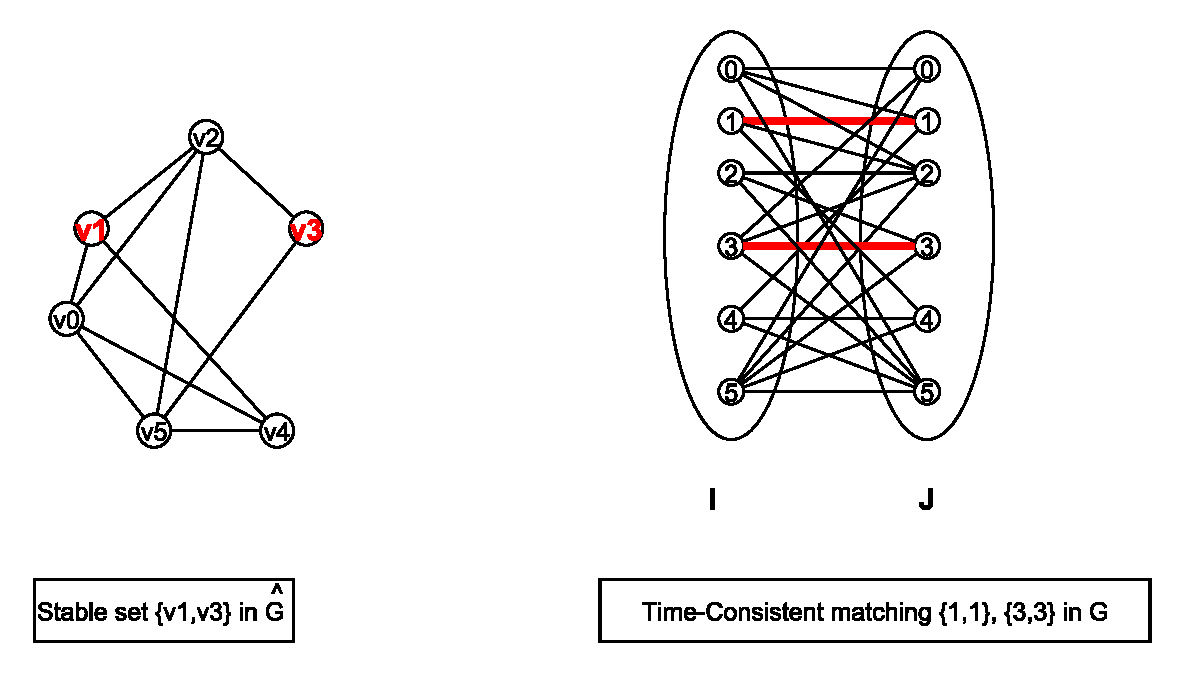
\includegraphics[height=60mm]{ConsistCompl.pdf}}
	\caption[]{Transformation from a stable set in $H$ to a Time-consistent matching in G}
	\label{TIM}
\end{figure}
%

In the last part of this subsection, assume that the weight function satisfies the \emph{(SA)} property:
$$ \begin{array}{lr}
\forall j_1, j_2, j_3 \in \llbracket 0, M \rrbracket, j_1 < j_2 < j_3 \Rightarrow w(j_1, j_2) + w(j_2, j_3) \leq w(j_1, j_3) & \textrm{(SA)}
\end{array} $$ 
%
Then, if the pairs $\{(i_1, j_1), (i_2, j_2) \}$ and  $\{(i_2, j_2), (i_3, j_3) \}$ are time-inconsistent
for some $ 0\leq j_1 < j_2< j_3 \leq M$ and $ 0\leq i_1 < i_2 < i_3 \leq N-1$, then 
the pair $\{(i_1, j_1), (i_3, j_3) \}$ is also time-inconsistent.

With respect to the (SA)-property, valid constraints can be obtained as in Section~\ref{Non_crossing_matchings}.
First, let us complete the directed acyclic graph $H$ of Section~\ref{Non_crossing_matchings}  as follows.
For any $j < j'$ such that $w(j, j') \geq 2$, we add
 the arcs $((i' ,j'), (i,j))$ for $ \max(0, i' - w(j, j') +1) \leq i \leq i'-1, 1 \leq i' \leq N-1$.
 Denote by $H_\textrm{tc}$ this modified graph, by $A^+(H_\textrm{tc})$ the set of the new arcs, and
 by ${\cal P}_\textrm{tc}$ the set of  paths $P$ of origin $(0, M)$ and end $(N-1, 0)$ in $H_\textrm{tc}$.
%and by $E(P)$ the edges of $E$ that correspond to vertices of $P$.

So, for a maximal path $P \in {\cal P}_\textrm{tc}$,  the constraint 
\begin{eqnarray}
 \sum_{(i, j) \in E(P)} U_{i,j} \le 1 &\label{clique_timecons_P}
\end{eqnarray}
is called the {\it time-consistent} constraint associated to $P$. 
%%%%%%%%
\begin{lem}\label{lem_arc_time}
Let $(i_0', j_0') $  and $(i_0, j_0) $ be two vertices of $H_\textrm{tc}$ such that
$i_0' > i_0 $ and $j_0' > j_0 $. If there is a path in $H_\textrm{tc}$
from $(i_0', j_0') $ to $(i_0, j_0) $, then the arc 
$((i_0', j_0') , (i_0, j_0)) $ exists in $A^+(H_\textrm{tc})$.
\end{lem}
\begin{proof}
Consider two vertices $(i_0', j_0') $ and $(i_0, j_0) $ with $i_0' > i_0 $ and $j_0' > j_0 $
that are connected by a path $P$ in $H_\textrm{tc}$.
By construction of $H_\textrm{tc}$, it can be seen that $j_0' \geq j \geq  j_0 $
for all node $(i, j)$ in $P$.

Now, moving backwards along $P$ from $(i_0, j_0) $, we collect any arc 
$a= ((i',j'),(i,j))$ of $A^+(H_\textrm{tc})$ which satisfies
$i' <i_0'$. The collecting process is stopped when an arc $a_1= ((i_1',j_1'),(i_1,j_1))$
is found with $i_1' \geq i_0'$ for the first time.

Consider the sequence $ ((i_1',j_1'),(i_1,j_1)), ((i_2',j_2'),(i_2,j_2)), \dots ((i_q',j_q'),(i_q,j_q))$
of the arcs selected by the above procedure for some integer $q \ge 1$.
We have that 
\begin{itemize} 
\item [-] $ i_1' \geq i_0'$, $i_k' < i_0', k=2, \dots q$, $i_q \leq i_0$,
\item [-] $i_k < i_k', k=1, \dots q$,
\item [-] the intervals $[i_k,i_k'], k=1, \dots q$ cover the interval $[i_0,i_0']$.
\end{itemize}

By construction of $A^+(H_\textrm{tc})$, it is known that
\begin{displaymath}
\begin{array}{lcr}
i_1 + w(j_1, j_1') &> & i_1', \\
i_2 + w(j_2, j_2') & >& i_2', \\
\dots \\
i_q + w(j_q, j_q') & >& i_q'. 
\end{array}
\end{displaymath}
Thus 
$$ \sum_{k=1}^{q}{w(j_k, j_k') } > i_1' -  i_1 + i_2' - i_2 + \dots i_q' - i_q \geq i_0' - i_0.$$

As  $j_0' \geq j_1' > j_1 > j_2' >j_2 \dots > j_q' >j_q \geq j_0$,
by the (SA) property, we deduce that  $ w(j_0, j_0')  > i_0' - i_0$.
This implies that the arc $((i_0', j_0') , (i_0, j_0)) $ is in  $A^+(H_\textrm{tc})$.
\end{proof}


%%%%%%
%\begin{figure}[!ht]
	%\centerline{
		%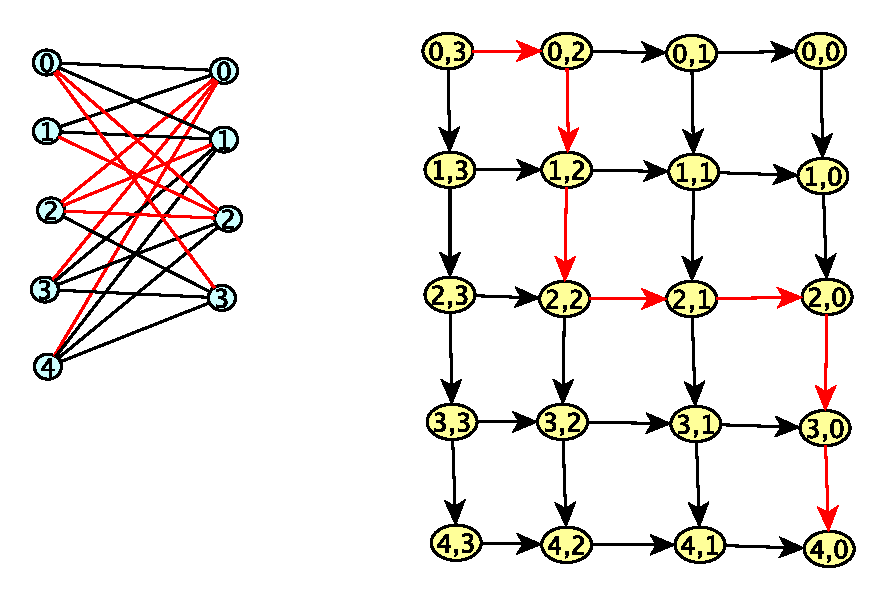
\includegraphics[height=40mm]{NonCrossingM.pdf}}
	%\caption[]{A path in $H$ associated to a set of crossing edges in $G$.}
	%\label{NCM}
%\end{figure}
%%%%%%%%
\begin{lem}\label{lem_timecons}
For any maximal path $P$ in $H_\textrm{tc}$, the time-consistent constraint induced by $P$ is valid for $MILP_{SMEPC}$.
\end{lem}
\begin{proof}
Consider a maximal path $P =( (i_1, j_1), (i_2, j_2), \dots (i_{Q-1}, j_{Q-1}), (i_{Q}, j_{Q}))$
 of ${\cal P}_\textrm{tc}$
with $(i_1, j_1)=(0,M)$ and $(i_{Q}, j_{Q})=(N-1, 0)$. 
Suppose that a time-consistent matching $C(U)$ has a non empty
intersection with $E(P)$, for some feasible $U$ of $MILP_{SMEPC}$. 
Let $(i_{k_0},j_{k_0}), 1 \le k_0 \le Q,$ be the first edge of $E(P)$ belonging to $C(U)$.
Suppose that there is an other edge   $(i_{k_1},j_{k_1}), 1 \le k_0 < k_1 \le Q$ in $C(U)$. This implies that $ i_{k_0} \neq i_{k_1}$ and
$ j_{k_0} > j_{k_1}$ since $C(U)$ is a matching. Moreover, as $C(U)$ is also non-crossing,
by construction of $A^+(H_\textrm{tc})$, 
we have $ i_{k_0} > i_{k_1}$. 
Thus, the two nodes are in $P$ and, by~Lemma~\ref{lem_arc_time}, the
arc $a=((i_{k_0},j_{k_0}), (i_{k_1},j_{k_1})) $ belongs to  $A^+(H_\textrm{tc})$. 
Therefore, the edges $(i_{k_0},j_{k_0})$ and $(i_{k_1},j_{k_1})$
are time-inconsistent, a contradiction.
%Then the path $P'$ obtained from $P$
%by replacing the sub-path between $(i_{k_0},j_{k_0})$ and $ (i_{k_1},j_{k_1}) $ by $a$
%generates a constraint of type~(\ref{clique_timecons_P}) which is violated by $C(U)$, a contradiction.
\end{proof}

In the same way as Section~\ref{NonCross}, it can be seen that the polytope $Q_{t_c}$, defined by inequalities (\ref{positivite}) and (\ref{clique_timecons_P}), for any path $P \in {\cal P}_\textrm{tc}$, describes the convex hull of characteristic vectors of time-consistent matchings, when $(SA)$ property is satisfied.

For $0\le j<j'\le M$, let $\tilde{w}(j, j')=\sum_{k=j+1}^{j'-1} t_k, j'>j+1$ and $0$ otherwise. It is
obvious  that the values $\tilde{w}(j,j')$ satisfy the $(SA)$ property and allow a time-consistent constraint generation, which is tested in the experimental part.

%%%%%%%%%%%%%%%%%%%%%%%%%%%%%%%%%%%%%%%%%%%%%%%
%\section{Separation procedures }\label{sec5}
%%%%%%%%%%%%%%%%%%%%%%%%%%%%%%%%%%%%%%%%%%%%%%%
\section{Computational results }\label{sec6}
\subsection{Computation environment}
The experiments are performed on a computer with AMD EPYC 7H12 64-Core processor, and 
are running under Gnu/linux Ubuntu 20.04.2. 
 CPLEX 12.10 is used in a single-thread mode with all its parameters  set to their default values. 
The maximum CPU time is fixed to 1 hour.
\subsection{Description of instances}
All series of  experiments concern the instances presented in Table \ref{tab:inst} with the following notations:

\begin{itemize}
\item num : the number of the instance,
 \item $M$: number of stations,
 \item $N$: number of production periods,
 \item $p$: duration of one production period,
 \item $H_0$: initial micro-plant hydrogen load,
  \item $C^{\textrm{MP}}$: micro-plant tank capacity,
 \item $E_0$: initial vehicle hydrogen load,
 \item $C^{\textrm{Veh}}$: vehicle tank capacity,
    \item LTour : duration of the tour without refueling,
    \item ETour : consumed volume without refueling.
\end{itemize}

The instances are generated as follows:
\begin{itemize}
\item $N, M$ and $p$ are fixed. 
\item The stations, $Depot$ and the Micro-Plant are randomly generated as points of a square in $\mathbb{R}^2$.
\item  $d_j$, $d^*_j$ and $t_j$, $e_j$, $\epsilon_j$, $\epsilon^*_j$, respectively correspond to Euclidean distance and Manhattan distance rounded, in such a way they take integral values.
\item $C^{MP}$, $C^{Veh}$ and $TMax$ are fixed in such a way the existence of a feasible solution is ensured.
 \item Finally, the activation cost  $Cost^F$ is set to $20$. 
Values of production costs $Cost^V_i$ $i = 0,\dots,N -1$, are independently uniformly generated in  $\llbracket 1, 10 \rrbracket$.
\end{itemize}

\begin{table}[H]
  \centering
  \caption{Instances}
	\small{
    \begin{tabular}{|r|rrrrrrrrr|}
    \toprule
    \textbf{num} &$\mathbf{M}$ & $\mathbf{N}$ & $\mathbf{p}$ &  $\mathbf{H_0} $ & $\mathbf{C^{MP}}$ & $\mathbf{E_0}$ & $\mathbf{C^{Veh}}$ & \textbf{LTour} & \textbf{Etour} \\
    \midrule
    1&8     & 20    & 4        & 6     & 25    & 8     & 12    & 20    & 20 \\
   2& 8     & 25    & 4        & 5     & 20    & 8     & 10    & 25    & 26 \\
   3& 8     & 40    & 5       & 10    & 70    & 20    & 30    & 44    & 50 \\
    4     &10    & 36    & 2     &  8     & 25    & 9     & 12    & 36    & 38 \\
    5     &10    & 50    & 4     &  6     & 40    & 10    & 20    & 50    & 54 \\
    6     &10    & 94    & 1     &  3     & 30    & 4     & 15    & 47    & 52 \\
    7     &12    & 32    & 4     &  0     & 50    & 4     & 25    & 63    & 68 \\
    8     &12    & 50    & 4     &  3     & 36    & 3     & 18    & 50    & 58 \\
    9     &15    & 160   & 4     &  8     & 240   & 20    & 120   & 426   & 556 \\
    10    &20    & 108   & 10    &  20    & 390   & 10    & 190   & 716   & 894 \\
    11    &10    & 80    & 2     &  10    & 40    & 10    & 20    & 38    & 38 \\
    12    & 15    & 327   & 4     & 20    & 400   & 11    & 140   & 653   & 790 \\
    13    &20    & 180   & 6     &  3     & 500   & 20    & 170   & 718   & 834 \\
    14    &20    & 440   & 5     &  100   & 350   & 50    & 170   & 910   & 1164 \\
    15    &30    & 177   & 8     &  6     & 420   & 10    & 200   & 944   & 1188 \\
    16    &30    & 260   & 6     &  50    & 400   & 50    & 200   & 1034  & 1320 \\
    17    & 30    & 544   & 4     & 10    & 560   & 15    & 250   & 1088  & 1382 \\
    18    & 50    & 265   & 10    & 6     & 400   & 9     & 200   & 1764  & 2216 \\
    19    & 50    & 500   & 8     & 100   & 420   & 50    & 180   & 1565  & 2000 \\
    20    &70    & 328   & 10    &  15    & 550   & 25    & 270   & 2183  & 2766 \\
    21    & 30    & 1100  & 2     & 100   & 400   & 80    & 200   & 1097  & 1342 \\
     22    &30    & 1200  & 2     & 100   & 400   & 70    & 200   & 957   & 1200 \\
   23    & 50    & 634   & 6     &  50    & 300   & 50    & 150   & 1542  & 1938 \\
    24    & 50    & 850   & 4     & 20    & 400   & 50    & 180   & 1941  & 2500 \\
    25    &50    & 1125  & 4     &  20    & 700   & 50    & 280   & 1718  & 2128 \\
    26    & 70    & 383   & 8     &  20    & 760   & 15    & 240   & 2039  & 2590 \\
    27    & 70    & 683   & 8     & 8     & 850   & 14    & 370   & 2185  & 2826 \\
     28    &70    & 984   & 6     & 50    & 750   & 40    & 250   & 2340  & 2926 \\
    29    &100   & 651   & 8     &  100   & 600   & 60    & 200   & 3471  & 4360 \\
    30    &100   & 800   & 10    &  100   & 950   & 100   & 430   & 3095  & 3796 \\
    \bottomrule
    \end{tabular}%
		}
  \label{tab:inst}%
\end{table}%
\subsection{Results for the linear relaxation $RMILP_{SMEPC}$ }

Our first experiments concern the linear relaxation $RMILP_{SMEPC}$. We study the contribution of   valid inequalities given in Section \ref{sec4}. In each case, the optimal objective value, the CPU time and the gap to the optimal solution of the $MILP_{SMEPC}$, if it exists or to the best bound, otherwise, are given.  Table \ref{tab:frac1} presents the results for:
\begin{itemize}
\item (LR): $RMILP_{SMEPC}$, the linear relaxation alone. 
\item  (LR)+( STC): $RMILP_{SMEPC}$, when only the simple time constraints are added.
 \item  (EC1+EC2):  incorporate the energy constraints EC1 and EC2 to  (LR)+( STC). 
 \item  (EC3): (LR)+( STC) with energy constraints EC3. 
\item  All energy: (LR)+( STC) with energy constraints EC1, EC2 and EC3.
 \end{itemize}
 For each case, we give the following results are specified
 \begin{itemize}
\item $TT$ : total CPU time in seconds.
\item $obj$ : optimal value of the linear program.
%\item $GapI$ : the relative error between the upper bound (the
%optimal solution if the problem is solved to optimality)
%and the lower bound obtained. The instances indicated with "**" are those whose CPU time exceeded 1h without obtaining an upper bound. We indicate in italic, the instances which are not solved to optimality.
\item $GapF$ : percentage of the relative error between the best feasible solution (optimal solution if the problem has been solved to optimality) and the optimal objective value of the linear relaxation. The instances indicated with "**" are those whose CPU time has exceeded 1h.
\end{itemize}
%%%%%%%%%%%%%%%%%%%%%%%%%%%%%%%%%%%%%%%%%%%%%%%%
\begin{table}[H]
  \centering
	\small
  \caption{The linear relaxation $RMILP_{SMEPC}$ and the effects of simple time constraints}
		\begin{tabular}{|r|rrr|rrr|}
    \toprule
    \multicolumn{4}{c}{\textbf{LR}}              & \multicolumn{3}{c}{\textbf{LR + STC}} \\
    \midrule
    \textbf{num} & \textbf{obj} & \textbf{TT} & \textbf{GapF} & \multicolumn{1}{r}{ \textbf{obj}} & \textbf{TT} & \textbf{GapF} \\
    \midrule
    1     & 44.15 & 0.0      & 66.29 & 68.18 & 0.0      & 47.95 \\
    2     & 36.94 & 0.0        & 75.53 & 64.89 & 0.1       & 57.02 \\
    3     & 30.93 & 0.1       & 78.52 & 79.51 & 0.1       & 44.79 \\
    4     & 45.34 & 0.0       & 67.62 & 82.52 & 0.0       & 41.06 \\
    5     & 46.42 & 0.1       & 71.17 & 97.27 & 0.0     & 39.58 \\
    6     & 41.26 & 0.1       & 76.82 & 97.79 & 0.1     & 45.06 \\
    7     & 52.00 & 0.1      & 76.57 & 124.84 & 0.0       & 43.77 \\
    8     & 39.97 & 0.0      & 79.18 & 96.43 & 0.0     & 49.78 \\
    9     & 80.16 & 0.1     & 87.55 & 523.61 & 0.1    & 18.69 \\
    10    & 59.41 & 0.1       & 94.78 & 883.52 & 0.1      & 22.43 \\
    11    & 27.60 & 0.1      & 79.40 & 78.80 & 0.0       & 41.19 \\
    12    & 37.90 & 0.2     & 95.84 & 717.05 & 0.4      & 21.38 \\
    13    & 33.34 & 0.1     & 96.51 & 794.71 & 0.2      & 16.87 \\
    14    & 69.60 & 0.4     & 94.93 & 1049.27 & 1.3      & 23.52 \\
    15    & 68.84 & 0.2      & 94.89 & 1114.54 & 0.3     & 17.20 \\
    16    & 62.16 & 0.3       & 95.19 & 1120.57 & 0.4      & 13.20 \\
    17    & 49.10 & 0.5      &\it{ 96.18} & 1155.17 & 2.4       &  10.10 \\
    18    & 125.35 & 0.6       & \it{ 94.72} & 1942.44 & 0.8       &  18.14 \\
    19    & 137.60 & 1.4     & \it{ 93.84 }& 1826.41 & 5.0       &  18.17 \\
    20    & 106.04 & 1.0      & \it{ 96.02} & 2311.54 & 1.5       &  13.30 \\
    21    & 70.42 & 3.3     & \it{ 95.01} & 1240.39 & 10.6    &  12.15 \\
    22    & 60.27 & 2.7    & \it{ 95.51 }& 1106.55 & 7.0    &  17.54 \\
    23    & 134.63 & 2.2    & \it{ 94.80} & 1910.07 & 7.6      &  26.28 \\
    24    & 135.81 & 3.2      & \it{ 95.18} & 2268.60 & 10.8     &  19.55 \\
    25    & 75.16 & 7.3     & \it{ 96.35 }& 1864.20 & 17.3    &  9.37 \\
    26    & 15.78 & 2.8      &\it{  99.33} & 2088.61 & 4.0      & 1 1.95 \\
    27    & 76.73 & 2.9     & \it{ 96.94} & 2268.94 & 7.7      &  9.50 \\
    28    & 90.08 & 7.3      &\it{  98.02} & 2661.38 & 21.2     &  41.43 \\
    29    & 175.85 & 6.2     & **    & 3759.44 & 13.9    & ** \\
    30    & 72.49 & 3.4     &  98.62 & 3191.14 & 8.4      &  39.07 \\
    \bottomrule
    \end{tabular}%
  \label{tab:frac1}%
\end{table}%
%%%%%%%%%%%%%%%%%%%%%%%%%%%%%%%%%%%%%%%%%%%%%%%%%%%%%%%%%%%%%%%%%%%%%%%%%%%%%%%%%%%%%%%%%
\begin{table}[H]
  \centering
  \small
  \caption{The linear relaxation $RMILP_{SMEPC}$ and the effects of energy constraints}
    \begin{tabular}{r|rrr|rrr|rrr|rrr|}
    \toprule
    &\multicolumn{3}{c|}{\textbf{LR + STC}} & \multicolumn{3}{c|}{\textbf{EC1+EC2}}&\multicolumn{3}{c|}{\textbf{EC3}}&\multicolumn{3}{c|}{\textbf{All Energy}} \\
    \midrule
    \textbf{num} & \textbf{obj} & \textbf{TT} & \textbf{GapF} & \textbf{obj} & \textbf{TT}  & \textbf{GapF} & \textbf{obj} & \textbf{TT} &  \textbf{GapF} &\textbf{obj} & \textbf{TT} & \textbf{GapF} \\
    \midrule
    1     & 68.18 & 0.0   & 47.95  & 68.18 & 0.1  & 47.95  & 79.5258 & 0.1   & 39.29 & 81.77 & 0.0   & 37.58 \\
    2     & 64.89 & 0.1   & 57.02  & 77.25 & 0.0   & 48.84  & 73.6146 & 0.1    & 51.25 & 87.58 & 0.1   &42.00 \\
    3     & 79.51 & 0.1   & 44.79 & 85.18 & 0.1   & 40.85 & 80.7294 & 0.1     & 43.94 & 86.48 & 0.1   & 39.94 \\
    4     & 82.52 & 0.0   & 41.06 &  95.13 & 0.0   &  32.05& 89.1597 & 0.1    & 36.31 & 103.15 & 0.1  & 26.32 \\
    5     & 97.27 & 0.0   & 39.58 & 102.97 & 0.1   & 36.04 & 102.194 & 0.1    & 36.53 & 108.52 & 0.1   &  32.60 \\
    6     & 97.79 & 0.1   & 45.06 &  117.31 & 0.1   &  34.09  & 115.567 & 0.1    & 35.07 & 134.76 & 0.1  & 24.29 \\
    7     & 124.84 & 0.0   & 43.77 &  136.46 & 0.0   &  38.53  & 142.594 & 0.1  &  35.77 & 155.67 & 0.1   & 29.88\\
    8     & 96.43 & 0.0   & 49.78 &  109.33 & 0.1   & 43.06  & 110.698 & 0.1  & 42.34 & 125.99 & 0.1 & 34.38 \\
    9     & 523.61 & 0.1   & 18.69 & 536.21 & 0.1   &16.74 & 570.346 & 0.2   & 11.44 & 584.29 & 0.3   &  9.27 \\
    10    & 883.52 & 0.1   & 22.43 &  909.99 & 0.1   &  20.11& 963.463 & 0.2 & 15.41 & 984.70 & 0.3   & 13.55  \\
    11    & 78.80 & 0.0   & 41.19 & 88.46 & 0.0   & 33.99 & 91.3411 & 0.1  & 31.84 & 102.31 & 0.1   & 23.65 \\
    12    & 717.05 & 0.4   & 21.38 &  732.63 & 0.2   &  19.67 & 830.481 & 0.9 & 8.94  & 846.13 & 0.7   & 7.22 \\
    13    & 794.71 & 0.2   & 16.87 & 807.91 & 0.2   &  15.49  & 854.829 & 0.4  & 10.58 & 863.65 & 0.2   & 9.66 \\
    14    & 1049.27 & 1.3   & 23.52 &  1073.81 & 0.5   &  21.73  & 1218.37 & 2.8   & 11.20 & 1246.31 & 1.8&  9.16 \\
    15    & 1114.54 & 0.3   & 17.20 & 1135.81 & 0.2   & 15.62& 1183.52 & 0.4     & 12.07 & 1200.46 & 0.5 &  10.81 \\ 
    16    & 1120.57 & 0.4   & 13.20 & 1149.03 & 0.4   & 11.00& 1160.43 & 1.7 & 10.11 & 1189.91 & 1.7  & 7.83 \\ 
    17    & 1155.17 & 2.4   & 10.10 & 1172.22 & 1.2   &  8.78  & 1196.6 & 3.9  & 6.88  & 1209.30 & 7.0   & 5.89 \\
    18    & 1942.44 & 0.8   & 18.14 &  1995.63 & 0.8   &  15.90 & 2059.16 & 1.1 & 13.23 & 2110.38 &1.7 &11.07 \\ 
    19    & 1826.41 & 5.0   & 18.17 & 1856.81 & 3.7   &  16.81 & 1902.51 & 11.0  & 14.76 & 1932.25 & 21.6  & 13.43 \\
    20    & 2311.54 & 1.5   & 13.30 & 2351.12 & 0.9   & 11.81    & 2342.78 & 7.1 & 12.12 & 2382.36 & 16.3& 10.64 \\
    21    & 1240.39 & 10.6  & 12.15 &  1263.48 & 2.3   & 10.52& 1316.83 & 18.7  & 6.74  & 1340.30 & 7.6   &  5.08 \\ 
    22    & 1106.55 & 7.0   & 17.54 &1129.40 & 4.4   & 15.84 & 1228.15 & 20.0 & 8.48  & 1252.20 & 34.8  &  6.69 \\
    23    & 1910.07 & 7.6   & 26.28 &  1971.99 & 4.5   &23.89 & 2316.46 & 8.7  & 10.60 & 2387.33 & 12.3  & 7.86 \\ 
    24    & 2268.60 & 10.8  & 19.55 &  2325.79 & 2.4   &  17.53 & 2561.57 & 16.7 & 9.16  & 2621.32 & 14.1  &  7.05 \\
    25    & 1864.20 & 17.3  & 9.37  &  1876.85 & 3.9   & 8.76  & 1944.81 & 42.0 & 5.45  & 1956.51 & 83.2  & 4.89 \\
    26    & 2088.61 & 4.0   & 11.95 &  2151.98 & 1.0   &  9.28& 2115.79 & 8.3  & 10.80 & 2176.70 & 8.3 & 8.23 \\ 
    27    & 2268.94 & 7.7   & 9.50  & 2289.61 & 6.2   &  8.67& 2292.71 & 17.3  & 8.55 & 2309.62 & 27.9& 7.87 \\ 
    28    & 2661.38 & 21.2  & 41.43 & 2685.29 & 15.3  &  40.90 & 2815.69 & 52.5 & 38.03 & 2839.81 & 119.2 &37.50 \\
    29    & 3759.44 & 13.9  & **    & 3813.40 & 12.1  &  **& 3914.15 & 30.8   & **    & 3970.15 & 101.5& ** \\ 
    30    & 3191.14 & 8.4   & 39.07 &  3224.40 & 7.6   & 38.43& 3233.22 & 8.0  & 38.26 & 3265.79 & 64.1  &37.64 \\ 
    \bottomrule
    \end{tabular}%
  \label{tab:frac2}%
\end{table}%
%%%%%%%%%%%%%%%%%%%%%%%%%%%%%%%%%%%%%%%%%%%%%%%%%%
\subsection{Results for Mixed integer linear programming $MILP_{SMEPC}$ }

 \begin{itemize}
\item $TT$: total CPU time in seconds.
\item $LB$ and $UB$: Lower and Upper bounds  of the mixed integer linear program respectively. The upper bound is the best integer feasible solution.
%\item $GapI$ : the relative error between the upper bound (the
%optimal solution if the problem is solved to optimality)
%and the lower bound obtained. The instances indicated with "**" are those whose CPU time exceeded 1h without obtaining an upper bound. We indicate in italic, the instances which are not solved to optimality.
\item $GapMI$: percentage of the relative error between the lower bound and the upper bound. 
The instances indicated with "**" are those whose CPU time has exceeded 1h and no upper bound was obtained after this time. The instances that could not be solved to optimality but for which an upper bound is reached within 1h have their gap indicated in italic.
\end{itemize}
\begin{table}[H]
  \centering
  \small
  \caption{ Cplex +STC, time limit = 1h}
    \begin{tabular}{|r|rrrrr|}
    \toprule
    \multicolumn{5}{c}{ STC}                       &  \\
    \midrule
    \textbf{num} &  \textbf{LB} & \textbf{UB}  & \textbf{nodes} & \textbf{TT} & \textbf{GapMI} \\
    \midrule
    1     & 131   & 131   & 1123  & 1.0   & 0.00 \\
    2    & 151   & 151   & 2701  & 2.3   & 0.00 \\
    3     &144   & 144   &  1699  & 2.3   & 0.00 \\
    4     & 140   & 140   & 3896  & 3.9   & 0.00 \\
    5      & 161   & 161   &  1252  & 1.7   & 0.00 \\
    6     &178   & 178   & 20527 & 33.8  & 0.00 \\
    7     &  222   & 222   &  4683  & 3.5   & 0.00 \\
    8     & 192   & 192   &12263 & 25.5  & 0.00 \\
    9     &644   & 644   &7693  & 17.7  & 0.00 \\
    10    &  1139  & 1139  &  46518 & 37.7  & 0.00 \\
    11    &  134   & 134   & 5870  & 7.6   & 0.00 \\
    12    &  912   & 912   & 97686 & 458.2 & 0.00 \\
    13    &  956   & 956   & 24101 & 48.6  & 0.00 \\
    14    & 1372  & 1372  &  487725 & 2629.5 & 0.00 \\
    15    &  1346  & 1346  & 678590 & 1188.2 & 0.00 \\
    16    & 1291  & 1291  &  620432 & 1620.9 & 0.00 \\
    17    &1246.49 & 1285  & 242500 & 3600.1 & {\it 3.00} \\
    18    &  2208.43 & 2456  &198780 & 3600.1 & {\it 10.08} \\
    19    &2038.48 & 2275  & 38496 & 3600.1 &  {\it 10.40} \\
    20    &  2416.31 & 2666  &165044 & 3600.1 & {\it 9.37} \\
    21    & 1353.44 & 1424  &  81490 & 3600.2 & {\it 4.96} \\
    22    &1253.15 & 1363  & 28400 & 3600.3 & {\it 8.06} \\
    23    & 2237.48 & **   & 30474 & 3600.1 & ** \\
    24     & 2572.50 & **    & 33718 & 3600.2 & ** \\
    25    & 1946.27 & **   & 6269  & 3600.2 & ** \\
    26    &  2175.70 & 2458  & 43231 & 3600.1 & {\it 11.48} \\
    27    & 2335.89 & 2507  &  23987 & 3600.2 & {\it 6.83} \\
    28    &2768.95 & 4544  & 5681  & 3600.5 & {\it 39.06} \\
    29    & 3941.23 & **    &18958 & 3600.3 & ** \\
   30    & 3269.36 & **    & 2726  & 3600.3 & ** \\
    \bottomrule
    \end{tabular}%
  \label{tab:ChSymStc}%
\end{table}%

%%%%%%%%%%%%%%%%%%%%%%%%%%%%%%%%%%%%%%%%%%%%%%%
\begin{table}[H]
  \centering
  \small
  \caption{Energy constraints}
    \begin{tabular}{|r|rrrr|rrrr|rrrr|}
    \toprule
    &\multicolumn{4}{c|}{\textbf{ EC1, EC2}}     & \multicolumn{4}{c|}{\textbf{ EC3}} & \multicolumn{4}{c|}{\textbf{ All energy}} \\
    \midrule
    \textbf{num} & \textbf{LB} & \textbf{UB}  & \textbf{TT} & \textbf{gapMI} &  \textbf{LB} & \textbf{UB}  &\textbf{TT} & \textbf{gapMI} &  \textbf{LB} & \textbf{UB}  &\textbf{TT} & \textbf{gapMI} \\
    \midrule
    1     & 131   & 131& 0.5   & 0  & 131   & 131&    0.5   & 0  & 131   & 131& 0.6   & 0\\
    2     & 151   & 151 & 1.3   & 0  & 151   & 151 & 1.9  & 0 & 151   & 151& 1.3   & 0 \\
    3     & 144   & 144 & 1.4   & 0 & 144   & 144     & 1.6   & 0 & 144   & 144& 1.3   & 0 \\
    4     & 140   & 140  & 5.8   & 0  & 140   & 140  & 2.2   & 0& 140   & 140& 2.3   & 0 \\
    5     & 161   & 161& 2.4   & 0     & 161   & 161 & 2.3   & 0 & 161   & 161 & 1.4   & 0\\
    6     & 178   & 178& 29.8  & 0   & 178   & 178  & 64.2  & 0 & 178   & 178 & 39.9  & 0 \\
    7     & 222   & 222&  1.7   & 0  & 222   & 222   & 0.8   & 0& 222   & 222& 0.9   & 0 \\
    8     & 192   & 192&  33.5  & 0  & 192   & 192   &29.4  & 0& 192   & 192 & 21.6  & 0 \\
    9     & 644   & 644 & 26.2  & 0   & 644   & 644   &  63.1  & 0 & 644   & 644  & 37.4  & 0\\
    10    & 1139  & 1139 &26.9  & 0   & 1139  & 1139  &35.7  & 0& 1139  & 1139  & 8.7   & 0 \\
    11    & 134   & 134& 7.1   & 0 & 134   & 134    &  6.7   & 0 & 134   & 134 & 4.9   & 0\\
    12    & 912   & 912&  326.7 & 0& 912   & 912     &  259.2 & 0 & 912   & 912& 231.4 & 0 \\
    13    & 956   & 956&  58.1  & 0   & 956   & 956  &  64.1  & 0& 956   & 956& 32.2  & 0 \\
    14    & 1372  & 1372&  192.1 & 0 & 1372  & 1372    &  1686.1 & 0& 1372  & 1372 & 885.8 & 0 \\
    15    & 1346  & 1346& 1321.3 & 0  & 1346  & 1346  & 1675.0 & 0 & 1346  & 1346& 677.5 & 0 \\
    16    & 1291  & 1291&  2543.8 & 0 & 1291  & 1291    & 3451.9 & 0 & 1291  & 1291& 869.8 & 0 \\
    17    & 1250.30 & 1288&3600.1 & {\it 2.93} & 1267.42 & 1285 & 3600.1 & {\it 1.37} & 1272.09 & 1288 & 3600.1 & {\it 1.24}\\
    18    & 2252.20 & 2408& 3600.1 & {\it 6.47}& 2317.26 & 2382  & 3600.1 & {\it 2.72} & 2322.5 & 2373& 3600.1 & {\it 2.13}\\
    19    & 2044.24 & 2374& 3600.2 & {\it 13.89}& 2083.45 & 2232& 3600.1 & {\it 6.66}& 2105.92 & 2247& 3600.3 & {\it 6.28} \\
    20    & 2446.70 & 2993&  3600.2 & {\it 18.25}& 2433.72 & 2713 & 3600.1 & {\it 10.29}& 2462.32 & 2780& 3600.2 & {\it 11.43} \\
    21    & 1364.40 & 1412& 3600.3 &{\it  3.37}  &  1363.56 & 1412& 3600.2 & {\it 3.43}& 1377.03 & **  & 3600.2 & ** \\
    22    & 1288.58 & 1352& 3600.2 & {\it  4.69} & 1297.89 & 1342 & 3600.2 & {\it  3.29} & 1310.74 & **& 3600.3 & ** \\
    23    & 2417.76 & 2648&3600.2 & {\it  8.69} & 2486.83 & 2591 & 3600.2 & {\it  4.02} & 2502.81 & **& 3600.2 & ** \\
    24     & 2635.35 & 3132& 3600.3 & {\it  15.86} & 2682.25 & 2820& 3600.2 & {\it  4.88} & 2723.43 & 2861 & 3600.3 & {\it  4.81}\\
    25    & 1975.89 & 2131 & 3600.4 & {\it  7.28} & 2010.29 & 2061 &3600.3 & {\it  2.46} & 2020.03 & 2057   & 3600.4 & {\it  1.80}\\
    26  & 2245.61 & 2396 & 3600.2 & {\it  6.28}& 2250.90 & 2372  & 3600.1 & {\it  5.11}  & 2299.79 & 2380& 3600.2 &{\it   3.37}\\
    27    & 2349.76 & **& 3600.4 & **  & 2349.96 & 2531  & 3600.3 & {\it  7.15}& 2349.6 & **    & 3600.4 & ** \\
    28    & 2812.58 & **  & 3600.5 &** & 2846.28 & **    &3600.3 & ** & 2870.28 & **& 3600.6 & ** \\
    29    & 3953.29 & **& 3600.5 & **  & 4044.89 & **  & 3600.3 & **& 4113.51 & ** & 3600.5 & ** \\
    30    & 3291.77 & **    &  3600.8 & ** & 3287.42 & 5237&  3600.4 & {\it  37.23}& 3311.99 & **   & 3600.8 & **  \\
    \bottomrule
    \end{tabular}%
  \label{tab:champEC}%
\end{table}%
%\break

%\subsection{ Conclusion on the numerical results}
Preliminary trials were done with the basic formulation of Section \ref{sec4} only.  Its weakness rapidly appeared
since CPLEX could not find  a feasible solution to the last fifteen  instances of Table \ref{tab:inst} after one hour
of CPU time. 
We then observe that with (STC) constraints, CPLEX can reach a feasible solution on half of these data sets.
This explains why  the reference formulation will  incorporate (STC) constraints.


%For the other instances numbered from 17 to 30, an upper bound is obtained after one hour in most cases. 

%The simple time constraints bring a clear improvement to the resolution both in the Mixed integer linear program or in its relaxation even if for 5 instances the upper bound is not reached after one hour. 

Let us examine before the linear relaxation. Tests are made with different sets of constraints to explore their efficiency in solving these instances.
In Table \ref{tab:frac1}, the first column confirms the deficiency of the initial formulation
due to the large gap with respect to the optimum integer solution. The second column shows us that the objective  value of $RMILP_{SMEPC}$ is less than 50\% of the optimum for most  of 50\% of the instances with regard to the reference formulation. The gap to the best upper bound for the difficult instances 17 to 30 even drops to 20\%. 
Table  \ref{tab:frac2} shows that these results are improved by adding the energy constraints. Specially, the  three sets (EC1), (EC2) and (EC3) of energy constraints put all together, give the best bounds in return for a moderate running time increase.

In the integer resolution  framework of the reference model, 
Tables \ref{tab:ChSymStc} and \ref{tab:champEC} show that sixteen instances out of the thirty tested are solved to optimality. These data sets can be considered  as  {\it easy }instances. The different sets of inequalities are successively put at stake  for testing their contributions.
We can note from Table \ref{tab:champEC}, that (EC1) and (EC2) energy constraints fail on only four instances whereas  the (EC3) constraints alone fail on two instances. 
Surprisingly, other constraints that seemed promising such as (\ref{struct_const}) and the antagonistic constraints, have no effect in improving the gap. A Branch-and-Cut procedure has been tested where the polynomial time separation algorithms proposed in Section~\ref{sec5} have been  implemented. 
But the results indicate that neither antagonistic  constraints nor time-consistent inequalities even violated at 0.1 have no impact on the objective value. The combinatorial nature of these inequalities does not help to solve the mixed integer linear program.

%We find the same observations in the case of the tests conducted for the mixed integer linear program.

%%%%%%%%%%%%%%%%%%%%%%%%%%%%%%%%%%%%%%%%%%%%%%%%%%%%%%%%%%%%%%%%%%%%%%%%%%%%%%%%
%\begin{table}[H]
  %\centering
  %\caption{The linear relaxation $RMILP_{SMEPC}$ and the effects of additional constraints}
	%\small{
    %\begin{tabular}{|r|rrr|rrr|rrr|rrr|}
    %\toprule
	%
    %\multicolumn{4}{c}{\textbf{LR}} & \multicolumn{3}{c}{\textbf{LR + STC}} &\multicolumn{3}{c}{\textbf{EC1+EC2}}&\multicolumn{3}{c}{\textbf{EC3}}\\
    %\midrule
    %\textbf{num} & \textbf{obj} & \textbf{TT} & \textbf{GapF} & \multicolumn{1}{r}{ \textbf{obj}} & \textbf{TT} & \textbf{GapF} & \multicolumn{1}{r}{ \textbf{obj}} & \textbf{TT} & \textbf{GapF} & \multicolumn{1}{r}{ \textbf{obj}} & \textbf{TT} & \textbf{GapF} \\
    %\midrule
    %1     & 44.15 & 0.0   &   66.29     & 68.18 & 0.0   &    & 68.18 & 0.1   & 0.00  & 79.5258 & 0.1   & 16.64   \\
    %2     & 36.94 & 0.0   &   75.53     & 64.89 & 0.1   &     &77.25 & 0.0   & 19.04 & 73.6146 & 0.1   & 13.44 \\
    %3     & 30.93 & 0.1   &    78.52      & 79.51 & 0.1   &     & 85.18 & 0.1   & 7.13  & 80.7294 & 0.1   & 1.54 \\
    %4     & 45.34 & 0.0   &     67.62   & 82.52 & 0.0   &     & 95.13 & 0.0   & 15.29 & 89.1597 & 0.1   & 8.05\\
    %5     & 46.42 & 0.1   &  71.17      & 97.27 & 0.0   &    & 102.97 & 0.1   & 5.86  & 102.194 & 0.1   & 5.06 \\
    %6     & 41.26 & 0.1   & 76.82   & 97.79 & 0.1   &      & 117.31 & 0.1   & 19.96 & 115.567 & 0.1   & 18.18 \\
    %7     & 52.00 & 0.1   &  76.57   & 124.84 & 0.0   &    & 136.46 & 0.0   & 9.31  & 142.594 & 0.1   & 14.22   \\
    %8     & 39.97 & 0.0   &   79.18      & 96.43 & 0.0   &      & 109.33 & 0.1   & 13.38 & 110.698 & 0.1   & 14.80\\
    %9     & 80.16 & 0.1   &  87.55    & 523.61 & 0.1   &     & 536.21 & 0.1   & 2.41  & 570.346 & 0.2   & 8.93 \\
    %10    & 59.41 & 0.1   &  94.78      & 883.52 & 0.1   &    & 909.99 & 0.1   & 3.00  & 963.463 & 0.2   & 9.05 \ \\
    %11    & 27.60 & 0.1   &  79.40     & 78.80 & 0.0   &    & 88.46 & 0.0   & 12.25 & 91.3411 & 0.1   & 15.91\\
    %12    & 37.90 & 0.2   &  95.84    & 717.05 & 0.4   &      & 732.63 & 0.2   & 2.17  & 830.481 & 0.9   & 15.82  \\
    %13    & 33.34 & 0.1   &  96.51    & 794.71 & 0.2   &     & 807.91 & 0.2   & 1.66  & 854.829 & 0.4   & 7.57 \\
    %14    & 69.60 & 0.4   & 94.93    & 1049.27 & 1.3   &      & 1073.81 & 0.5   & 2.34  & 1218.37 & 2.8   & 16.12\\
    %15    & 68.84 & 0.2   &  94.89    & 1114.54 & 0.3   &    & 1135.81 & 0.2   & 1.91  & 1183.52 & 0.4   & 6.19  \\
    %16    & 62.16 & 0.3   & 95.19     & 1120.57 & 0.4   &    & 1149.03 & 0.4   & 2.54  & 1160.43 & 1.7   & 3.56\\
    %17    & 49.10 & 0.5   & 96.18     & 1155.17 & 2.4   &    & 1172.22 & 1.2   & 1.48  & 1196.6 & 3.9   & 3.59 \\
    %18    & 125.35 & 0.6   & 94.72    & 1942.44 & 0.8   &     & 1995.63 & 0.8   & 2.74  & 2059.16 & 1.1   & 6.01 \\
    %19    & 137.60 & 1.4   & 93.84      & 1826.41 & 5.0   &    & 1856.81 & 3.7   & 1.66  & 1902.51 & 11.0  & 4.17   \\
    %20    & 106.04 & 1.0   & 96.02      & 2311.54 & 1.5   &     & 2351.12 & 0.9   & 1.71  & 2342.78 & 7.1   & 1.35 \\
    %21    & 70.42 & 3.3   &  95.01     & 1240.39 & 10.6  &     & 1263.48 & 2.3   & 1.86  & 1316.83 & 18.7  & 6.16\\
    %22    & 60.27 & 2.7   & 95.51    & 1106.55 & 7.0   &    & 1129.40 & 4.4   & 2.06  & 1228.15 & 20.0  & 10.99 \\
    %23    & 134.63 & 2.2   &  94.80      & 1910.07 & 7.6   &  & 1971.99 & 4.5   & 3.24  & 2316.46 & 8.7   & 21.28   \\
    %24    & 135.81 & 3.2   &  95.18     & 2268.60 & 10.8  & & 2325.79 & 2.4   & 2.52  & 2561.57 & 16.7  & 12.91  \\
    %25    & 75.16 & 7.3   &  96.35    & 1864.20 & 17.3  &   & 1876.85 & 3.9   & 0.68  & 1944.81 & 42.0  & 4.32   \\
    %26    & 15.78 & 2.8   &  99.33    & 2088.61 & 4.0   &     & 2151.98 & 1.0   & 3.03  & 2115.79 & 8.3   & 1.30 \\
    %27    & 76.73 & 2.9   & 96.94 & 2268.94 & 7.7   &    & 2289.61 & 6.2   & 0.91  & 2292.71 & 17.3  & 1.05 \\
    %28    & 90.08 & 7.3   &    98.02   & 2661.38 & 21.2  &   & 2685.29 & 15.3  & 0.90  & 2815.69 & 52.5  & 5.80 \\
    %29    & 175.85 & 6.2   &  **   & 3759.44 & 13.9  &   & 3813.40 & 12.1  & 1.44  & 3914.15 & 30.8  & 4.12   \\
    %30    & 72.49 & 3.4   &    98.62  & 3191.14 & 8.4   &    & 3224.40 & 7.6   & 1.04  & 3233.22 & 8.0   & 1.32 \\
    %
		%\bottomrule
    %\end{tabular}%
		%}
  %\label{tab:frac1}%
%\end{table}%

%%%%%%%%%%%%%%%%%%%%%%%%%%%%%%%%%%%%%%%%%%%%%%%
\section{Conclusion}\label{sec7}
A mixed integer linear programming formulation for the Synchronized Management Energy Production and Consumption problem ($SMEPC$) is given and several families of valid inequalities are proposed. The experimental tests show the necessity of adding some of these constraints to enhance the basic model.

However, we report that structural constraints do not allow us to obtain an efficient Branch-and-Cut algorithm without knowing the reason of this failure. 

The future work consists in introducing the optimization of  vehicle tour and integrating several vehicles.

\begin{thebibliography}{999}
\bibitem{Bend} F. Bendali, E. Mole Kamga, J. 
Mailfert, A.  Quilliot and H. Toussaint, {\it Synchronizing energy production and vehicle routing.} RAIRO-Oper. Res. 55 (2021) 2141-2163.
%\bibitem{Chan} C.C. Chan, {\it The state of the art of electric, hybrid, and fuel cell vehicles.} Proc. IEEE 95 (2007) 704-718.
\bibitem{Dekk} R.  Dekker , J.  Bloemhof,  I.  Mallidis,  {\it Operations Research for Green Logistics -An Overview of Aspects, Issues, Contributions and Challenges.}European Journal of operational Research 219 (2012) 671-679.
\bibitem{Deza} A. Deza, K. Huang, M. R. Metel, {\it Charging station optimization for balanced electric car sharing.} Discrete Applied Mathematics (2020), https://doi.org/10.1016/j.dam.2020.01.042
\bibitem{Erdo} S. Erdogan and E. Miller-Hooks, {\it A green vehicle routing problem.} Transp. Res. Part E: Logist. Transp. Rev. 109 (2012)100-114.
%\bibitem{Fran}  A. Franceschetti, E. Demir, D. Honhon, T. Van Woensel, G. Laporte and M. Stobbe, {\it A metaheuristic for the time dependent pollution-routing problem.} Eur. J. Oper. Res. 259 (2017) 972-991.
\bibitem{Grim} C. Grimes, O. Varghese and S. Ranjan, {\it Light, Water, Hydrogen: The Solar generation of Hydrogen By Water Photo-electrolysis.} Springer-Verlag US (2008).
\bibitem{Koc} C. Ko\c{c}, O. Jabali, J. Mendoza and G. Laporte, {\it The electric vehicle routing problem with shared charging stations.} Int. Trans.
Oper. Res. 26 (2019) 1211-1243.
\bibitem{Lich} S. Licht, {\it Thermochemical and Thermal/Photo Hybrid Solar Water Splitting.} Springer New York, New York, NY (2008).
\bibitem{Ray} M. Raylan, S. Matos, Y. Frota and L. Satoru Ochi, {\it  Green vehicle routing and scheduling problem with split delivery.} Electron. Notes Disc. Math. 69 (2018) 13-20. Joint, EURO/ALIO, International Conference 2018 on Applied Combinatorial Optimization (EURO/ALIO 2018).
\bibitem{Sch} A. Schrijver, {\it Combinatorial Optimization: Polyhedra and Efficiency.} Vol. A, Chap. 14(2003).
%\bibitem{Laf} C. Laforest. {\it Private communication.}
	%\bibitem{Oos} M. Oosten,J.H.G.C Rutten and OF.C.R. Spieksma. {\it Disconnecting graphs by removing vertices: A polyhedral approach.} Statistica Neerlandica, 61(1),p:35-60, 2007.
\end{thebibliography}
%
\end{document}